\chapter{Component-Wise Performance Evaluation of OLTP Systems} \label{ch:looking_glass}

\section{Harizopoulos et al. ``OLTP through the Looking Glass, and What We Found There''} \label{sec:paper}

\subsection{Introduction}

    As a starting point for the search for optimization potentials of OLTP systems, Harizopoulos et al. in \cite{Harizopoulos:2008} have broken down the \emph{CPU time} used by the \emph{different components of a DBMS}. They stated that many of the features and guarantees provided by relational DBMS---which were mainly developed in the 1970's and 1980's---are not needed on \emph{modern hardware} and for many \emph{new applications}. Therefore, the CPU time consumed by the components responsible for realizing these features and guarantees can be seen as unnecessary overhead. Their work proves that significant performance improvements can be achieved with architectural changes for---what was called a few years later---NoSQL DBMS.

\subsection{Features and Guarantees Identified to be Unnecessary}

    \emph{Depending on the application}, one, some or all of the following features and guarantees typically provided by a relational DBMS have been identified as unnecessary by Harizopoulos et al.

    \begin{description}
        \item[Larger-Than-Memory Databases] Since \emph{database sizes grow more slowly than the available main memory}, it is no longer necessary to optimize a DBMS for DBs that are larger than the available main memory.
        \item[Multithreaded and Interleaved Execution] If transactions never block due to disk access latency, \emph{interleaved execution} using multithreading is no longer needed for good transaction throughput.
        \item[Strict Consistency and Transaction Support (and ACID in general)] For many new OLTP applications---especially in the area of distributed Internet services---the \emph{eventual consistency} will be sufficient. And a more complete approach---BASE (\textbf{B}asically \textbf{A}vailable, \textbf{S}oft state, \textbf{E}ventual consistency)---was later proposed by Pritchett in \cite{Pritchett:2008}.
        \item[Log-Based Recovery] On the one hand, some OLTP applications do \emph{not require recovery} at all, and on the other hand, recovery can be done from other sites of a \emph{cluster}.
    \end{description}

\subsection{Affected DBMS Components}

    The authors propose the removal of components from a DBMS to eliminate these features and guarantees along with the associated overheads.

    \begin{description}
        \item[Buffer Management] In-memory DBMSs simply allocate the DB in RAM.
        \item[Latching and Lock Management] Without support for multithreading and interleaved transaction execution, latching and locking is not required anymore.
        \item[Log Management] If crash recovery is required by the application, the required data can be provided by a \emph{replicated DBS}. However, replication using \emph{log-shipping} is not possible without a transaction log, so that other techniques must be used. The management of LSNs (log sequence numbers) is not necessary with a log-free DBMS.
        \item[B-Tree] B-tree indices are mostly \emph{optimized for disk-based use} \cite{Bayer:1970} and other data structures---like ART \cite{Leis:2013}---are better suited for in-memory DBMS. But using \emph{larger pages} can still improve the in-memory performance of B-trees. But for the evaluation in \cite{Harizopoulos:2008} the authors have simply \emph{hand-optimized} the B-tree code for the case of \emph{uncompressed integer keys} which are used throughout \textit{TPC-C}.
    \end{description}

\subsection{Performance Evaluation}

    They have \emph{analyzed these architectural changes quantitatively}, by taking the stock \textit{Shore Storage Manager}\footnote{\url{https://research.cs.wisc.edu/shore/}}\footnote{The \textit{Shore Storage Manager} (the remaining part of the \textit{Shore} DBMS) was derived from the \textit{EXODUS}. \textit{Shore} was later developed into \textit{Shore-MT}, the direct predecessor of \textit{Zero}, which is used throughout this thesis.} as a baseline and then \emph{gradually removing} the previously mentioned components. This gave them for each of these DBMS components the \emph{overhead} imposed on the overall system. They also applied some code optimizations to these components and to the remaining code, and tested the performance of a basic in-memory B-tree as a replacement for the DBMS. The used performance metrics are the \emph{instruction count} and \emph{CPU cycles} of the \textit{TPC-C} \emph{read-write transactions} NEW ORDER and PAYMENT.

\begin{@empty}
    \pgfplotsset{%
        every axis/.append style = {
            ybar stacked,
            ylabel near ticks,
            y label style = {font = \small},
            ylabel shift = -.5em,
            ymode = normal,
            ymin = 0,
            ytick style = {draw = none},
            yticklabel = {\prefix{\tick}},
            yticklabel style = {font = \scriptsize},
            ymode = normal,
            scaled y ticks = false,
            xmin = -0.25,
            xmax = 0.75,
            xtick = \empty,
            bar width = 0.5,
            ymajorgrids = false,
            width = .49\textwidth,
            height = .625\textheight
        }
    }

    \nottoggle{bwmode}{
        \tikzset{%
            a0/.style = {black, fill = cyan},
            a1/.style = {black, fill = cyan!75},
            a2/.style = {black, fill = cyan!50},
            a3/.style = {black, fill = cyan!25},
            b0/.style = {black, fill = magenta},
            b1/.style = {black, fill = magenta!66.66667},
            b2/.style = {black, fill = magenta!33.33333},
            c/.style = {black, fill = green!50},
            d/.style = {black, fill = white}
        }
    }{
        \tikzset{%
            a0/.style = {black, pattern color = black!25, pattern = {Lines[angle = 45, distance = 3pt]}},
            a1/.style = {black, pattern color = black!25, pattern = {Lines[angle = 45, distance = 6pt]}},
            a2/.style = {black, pattern color = black!25, pattern = {Lines[angle = 45, distance = 9pt]}},
            a3/.style = {black, pattern color = black!25, pattern = {Lines[angle = 45, distance = 12pt]}},
            b0/.style = {black, pattern color = black!25, pattern = {Lines[angle = -45, distance = 4pt]}},
            b1/.style = {black, pattern color = black!25, pattern = {Lines[angle = -45, distance = 8pt]}},
            b2/.style = {black, pattern color = black!25, pattern = {Lines[angle = -45, distance = 12pt]}},
            c/.style = {black, pattern color = black!25, pattern = horizontal lines},
            d/.style = {black, fill = white}
        }
    }
    
    \begin{figure}
        \centering
        \begin{tikzpicture}
            \begin{axis}[ylabel = {instructions},
                         ymax = 1730574.324]
                \node at (0.5, 60050.6757)  [draw = none]  {\footnotesize \SI{6.8}{\percent}};
                \node at (0.5, 413766.8919) [draw = none]  {\small\makecell[c]{buffer\\manager\\\footnotesize \SI{34.6}{\percent}}};
                \node at (0.5, 827280.4054) [draw = none]  {\small\makecell[c]{latching\\\footnotesize \SI{14.2}{\percent}}};
                \node at (0.5, 1095608.1082)[draw = none]  {\small\makecell[c]{locking\\\footnotesize \SI{16.3}{\percent}}};
                \node at (0.5, 1348226.3515)[draw = none]  {\small\makecell[c]{logging\\\footnotesize \SI{11.9}{\percent}}};
                \node at (0.5, 1591469.5945)[draw = none]  {\small\makecell[c]{Btree key\\\footnotesize \SI{16.2}{\percent}}};

                \node at (0, 0)             [draw = none, anchor = south, inner sep = 0.25mm] {\scriptsize useful work};
                \node at (0, 76520.270295)  [draw = none]                                     {\tiny remaining overhead};
                \node at (0, 120101.3514)   [draw = none, anchor = south, inner sep = 0.25mm] {\scriptsize Xactions};
                \node at (0, 287331.0811)   [draw = none]                                     {\scriptsize page access};
                \node at (0, 539949.3243)   [draw = none]                                     {\scriptsize small page};
                \node at (0, 707432.4324)   [draw = none, anchor = north, inner sep = 0.25mm] {\scriptsize dir lookup};
                \node at (0, 1275760.135)   [draw = none]                                     {\scriptsize LSN};
                \node at (0, 1370523.649)   [draw = none]                                     {\scriptsize main log};
                \node at (0, 1452364.865)   [draw = none, anchor = north, inner sep = 0.25mm] {\scriptsize disk log};
            
                \path[thick]    (-0.25, 120101.3514)     edge        (0.75, 120101.3514);
                \path[thick]    (-0.25, 707432.4324)     edge        (0.75, 707432.4324);
                \path[thick]    (-0.25, 947128.3784)     edge        (0.75, 947128.3784);
                \path[thick]    (-0.25, 1244087.838)     edge        (0.75, 1244087.838);
                \path[thick]    (-0.25, 1452364.865)     edge        (0.75, 1452364.865);
%                \path[thick]    (-0.25, 1730574.324)     edge        (0.75, 1730574.324);

                \addplot[c] coordinates         {(0, 32939.18919)};
                \addplot[d] coordinates            {(0, 87162.16216)};
                \addplot[a3] coordinates          {(0, 31418.91892)};
                \addplot[a2] coordinates          {(0, 271621.6216)};
                \addplot[a1] coordinates          {(0, 233614.8649)};
                \addplot[a0] coordinates             {(0, 50675.67568)};
                \addplot[b0] coordinates          {(0, 239695.9459)};
                \addplot[a0] coordinates             {(0, 296959.4595)};
                \addplot[b2] coordinates {(0, 63344.59459)};
                \addplot[b1] coordinates {(0, 126182.4324)};
                \addplot[b0] coordinates      {(0, 18750)};
                \addplot[a0] coordinates             {(0, 278209.4595)};
            \end{axis}
        \end{tikzpicture}
        \begin{tikzpicture}
            \begin{axis}[ylabel = {CPU cycles},
                         ymax = 3541922.952]
                \node at (0.5, 218679.1842) [draw = none] {\footnotesize \SI{12.3}{\percent}};
                \node at (0.5, 959695.6944) [draw = none] {\small\makecell[c]{buffer\\manager\\\footnotesize \SI{29.6}{\percent}}};
                \node at (0.5, 1665021.042) [draw = none] {\small\makecell[c]{latching\\\footnotesize \SI{10.2}{\percent}}};
                \node at (0.5, 2179993.525) [draw = none] {\small\makecell[c]{locking\\\footnotesize \SI{18.7}{\percent}}};
                \node at (0.5, 2879087.083) [draw = none] {\small\makecell[c]{logging\\\footnotesize \SI{21}{\percent}}};
                \node at (0.5, 3375000)     [draw = none] {\small\makecell[c]{Btree key\\\footnotesize \SI{8.1}{\percent}}};

                \path[thick]    (-0.25, 437358.3684)    edge        (0.75, 437358.3684);
                \path[thick]    (-0.25, 1482033.02)     edge        (0.75, 1482033.02);
                \path[thick]    (-0.25, 1848009.064)    edge        (0.75, 1848009.064);
                \path[thick]    (-0.25, 2511977.986)    edge        (0.75, 2511977.986);
                \path[thick]    (-0.25, 3246196.18)     edge        (0.75, 3246196.18);
%                \path[thick]    (-0.25, 3541922.952)    edge        (0.75, 3541922.952);

                \addplot[d] coordinates   {(0, 437358.3684)};
                \addplot[a0] coordinates    {(0, 1044674.652)};
                \addplot[b0] coordinates {(0, 365976.044)};
                \addplot[a0] coordinates    {(0, 663968.922)};
                \addplot[b0] coordinates {(0, 734218.1936)};
                \addplot[a0] coordinates    {(0, 295726.7724)};
            \end{axis}
        \end{tikzpicture}
        \caption[Results from \cite{Harizopoulos:2008}]{Number of CPU instructions and CPU cycles per \textit{TPC-C} NEW ORDER transaction measured by Harizopoulos et al. for \cite{Harizopoulos:2008}}
        \label{fig:lookingglassneworder}
    \end{figure}
\end{@empty}

    Figure \ref{fig:lookingglassneworder} shows their results for the NEW ORDER transaction. The number of CPU instructions executed during an average NEW ORDER transaction decreased by \SI{16.2}{\percent} after optimizing the search for uncompressed integer keys in \emph{B-tree} pages. Removing the I/O operations of the \emph{log manager} (\emph{disk log}), the generation of log records (\emph{main log}) and the maintenance of \emph{LSN} reduced the number of executed CPU instructions by a further \SI{11.9}{\percent} compared to the baseline. Removing calls to the \emph{lock manager} and the \emph{acquisition and release of latches} saved another \SI{16.3}{\percent} respective \SI{14.2}{\percent} of the instructions compared to the baseline. The authors achieved the greatest savings by removing parts of the \emph{buffer manager}. They removed the directory used to find storage structures like indexes on disk (\emph{dir lookup}), they increased the \emph{page size} from \SI{8}{\kilo\byte} to \SI{32}{\kilo\byte}, they removed the facilities used to access disk pages and find disk pages in the buffer pool (\emph{page access}) and they removed the transaction management (\emph{Xactions}). Their bare B-tree in main memory executed only a tiny fraction of the CPU instructions (\emph{useful work}) compared to the baseline.

    Fewer instructions do not result in the same degree of fewer CPU cycles. The optimizations the authors applied to \textit{Shore}'s \emph{B-tree} did not remove many \emph{CPU cache misses} and \emph{branch miss predictions} compared to their optimizations to other DBMS components, resulting in lower savings in required CPU cycles. The comparatively small fraction of instructions saved after removing \emph{transaction logging} resulted in a far greater proportion of CPU cycles saved because the logging code accessed \emph{many memory locations}. The remaining components require around two CPU cycles per instruction.

\subsection{Assessment of the Assumptions and Results}

    \begin{description}
        \item[Larger-Than-Memory Databases] The assumption that the DB of most OLTP applications fits in main memory is correct. But support for DBs larger-than-memory is still needed for \emph{embedded DBs}---such as those used by web browsers for managing browser history, cookies, or bookmarks---and for \emph{local copies} of production DBs on notebooks used to overcome network latency when working with e.g. GIS data in the home office.
        \item[Multithreaded and Interleaved Execution] Without multithreaded and interleaved execution, even a modern single CPU socket desktop PC with \emph{up to 64 CPU cores}\footnote{\url{https://www.amd.com/en/products/ryzen-threadripper}} cannot be utilized to the slightest degree.
        \item[Strict Consistency and Transaction Support (and ACID in general)] The idea that omitting transaction support and ACID guarantees is beneficial for most modern web applications led to the rise of \emph{NoSQL DBMSs in the 2000s}. These new systems were much more performant than traditional DBMSs and could be scaled horizontally. In the 2010s it was realized that the application development effort is higher when using a NoSQL DBMS and that relational DBMSs are possible with almost the performance and scalability of a NoSQL DBMS---\emph{NewSQL DBMSs} were born. An overview of the transition from NoSQL to NewSQL and a definition of NewSQL DBMSs can be found in \cite{Pavlo:2016}.
        \item[Performance Evaluation] The \textit{Shore Storage Manager} (as well as \textit{Zero}, which is used in his thesis) \emph{lacks the set-oriented layer} of a relational DBMS---it is therefore not fully representative for a traditional OLTP DBMS. But the greatest overhead of a relational DBMS should be below this layer, since it is mainly responsible for query optimization and compilation.\\
        The similar architectures of traditional DBMSs allow such a performance evaluation to be \emph{representative} to a certain extent, even if only one DBMS is examined. But evaluating multiple DBMSs would certainly have resulted in finding different optimization opportunities in these DBMSs, which would have led to different amounts of CPU instructions in the components.\\
        In general, the \textit{TPC-C} benchmark is a \emph{suitable benchmark} for evaluating the OLTP performance of a DBS. However, the two \emph{read/write transactions} selected by the authors (which account for \SI{88}{\percent} of the \textit{TPC-C} transactions) are not very representative for most web applications that use many \emph{read-only transactions}. Most importantly, the performance gain from eliminating \emph{transaction logging} is entirely based on the write accesses of these transactions. The standard transaction mixture of \textit{TPC-C}---or for a focus on Web applications more ORDER STATUS and STOCK LEVEL transactions---should be used for the performance evaluation.\\
        Harizopoulos et al. made it clear that they could not completely remove all components from \textit{Shore}, but that by removing them in a certain order helped to minimize the overhead caused by these leftovers. However, if one wants to optimize a component instead of removing it completely, breaking down the CPU time into the different components is not very helpful because it is \emph{too coarse}. A \emph{different order of component removals} would also lead to (slightly) different percentages of CPU time per DBMS component due to dependencies between different components. With the drawback of adding measurement overhead to the application under test---which slows it down and may distort the result---\emph{profiling and tracing software} can be used to obtain a code line-, function-, sub-component-, or component-wise breakdown of CPU cycles or other performance metrics.
        \item[Revisited] The measurements from \cite{Harizopoulos:2008} are \emph{repeated} in this chapter to address some of the problems of the original measurements. \emph{Multithreaded and interleaved} execution and \emph{all \textit{TPC-C} transactions} are considered. And instead of removing DBMS components, \emph{profiling and tracing} software on the baseline DBMS is used. The following section \ref{sec:profilingtracing} describes the technique and gives an overview of the software that can be used for this and describes in more detail the software that was used. Subsection \ref{subsec:looking_glass_single_threaded} gives results for single threaded DBS executions and subsection \ref{subsec:looking_glass_multi_threaded} discusses the multithreaded case. Section \ref{sec:looking_glass_optimizations} presents some optimizations that can be easily applied based on these measurements.
    \end{description}

\section{Profiling and Tracing} \label{sec:profilingtracing}

    The Oxford \textit{A Dictionary of Computer Science} \cite{Butterfield:2016} gives the following definitions:
    
    \begin{quote}
        \textbf{Profiling} ``Production of a histogram (or equivalent) concerning some aspect of a system. For example, an execution profile for a program might show the proportion of time spent in each individual procedure during a run of the program, while a statement profile might show the distribution of the statements in a program between the different kinds of statement provided by the language.''
    \end{quote}

    \begin{quote}
        \textbf{Trace Program} ``A program that monitors the execution of some software system and provides information on the dynamic behaviour of that system in the form of a trace, i.e. a report of the sequence of actions carried out. Typically a trace program will offer several options as to the kind of trace produced. For example, there may be options to produce a statement-by-statement trace, or to trace just those statements that alter the flow of control, or to trace changes to the value of a specific variable.''
    \end{quote}

    A \emph{program execution profile} is thus created by the aggregation of traces.

\subsection{Software}

    While many \emph{proprietary} performance analysis tools create execution profiles in one step---at least if one of the provided presets is suitable for the respective task---, the many \emph{free and open-source} programs only collect program traces. Analysis of the collected traces and profiling can be done using scripts \emph{written by the user} or \emph{shared online}. But for common profiling tasks free and open source GUI frontends are available, at least for the more popular programs. Some trace programs are also \emph{programmable}, which allows the user to perform more complex calculations during the tracing and to analyze the program execution in more detail, e.g. by reading variable values or function parameters, as is done in debugging.

    This subsection contains a brief description and/or potential sample analyses of free and open source performance analysis tools that could have been used (partially) for the measurements for section \ref{sec:looking_glass}. But for the simple analysis performed in section \ref{sec:looking_glass}, the less powerful \textit{Intel® VTune™ Profiler} was chosen because of its easy-to-use GUI and fast configuration. How to use it is described in more detail in subsection \ref{subsec:vtune}.

\paragraph{LTT}

    The \textit{Linux Trace Toolkit} is a \emph{simple} and \emph{not very configurable} \textit{Linux} kernel tracer that logs system calls, traps, interrupts, memory management events, etc. The traces are then displayed using a graphical visualizer.

\paragraph{LTTng}

    The \textit{Linux Trace Toolkit Next Generation}\footnote{\url{https://lttng.org/}} is a more sophisticated successor of \textit{LTT}. It can trace the \textit{Linux} kernel based on \emph{built-in tracepoints} and \emph{other instrumentation points}, but it can also be used to trace user programs that need to be prepared by inserting tracepoints. Tracing is managed in isolated tracing sessions, where different event rules can be set per session for kernel and user space tracing. A trace record containing, for example, the process ID, call stack or CPU performance counter values is produced whenever an active event rule is satisfied. To analyze the generated traces, tools like \textit{Babeltrace 2}\footnote{\url{https://babeltrace.org/}} are useful.

\paragraph{ftrace}

    \textit{ftrace}\footnote{\url{https://www.kernel.org/doc/Documentation/trace/ftrace.txt}} gives an insight into the operation of the \textit{Linux} kernel. It requires a \textit{Linux} kernel compiled with \textit{ftrace} capabilities enabled, and is configured using virtual files---it is not a command line application. Events that are used to create traces are kernel \emph{built-in static tracepoints}, \textit{kprobe} events, \textit{uprobe} events, or \emph{any function call within the kernel}. Tracing of specific events can be enabled in the configuration. It can also be used to measure certain \emph{latencies} within the kernel or to create a function graph. Tools for visualizing the not very human readable traces recorded by \textit{ftrace} are of course also available.

\paragraph{perf}

    \textit{perf} is a performance analysis tool built into \textit{Linux}, and it is probably the \emph{most commonly} used one on \textit{Linux}. It can create traces based on \emph{hardware events} (e.g. for microarchitecture-level analysis), \emph{low-level kernel events}, \emph{kernel tracepoints}, \emph{user-defined tracepoints} in user programs, dynamic \textit{kprobe} or \textit{uprobe} events, and a specific \emph{trace frequency}. \textit{perf} can create profiles that contain simple counter values, latencies aggregated per event, or human-readable aggregated call stacks with associated performance metrics.

\paragraph{DTrace}

    \textit{DTrace} is an open-source programmable tracing software that was originally released by \textit{Sun Microsystems} for \textit{Solaris} in 2005. Today, ports exist also for \textit{macOS}, \textit{Linux} and \textit{Windows}.

\begin{@empty}
    \begin{code}[h!]
        \begin{lstlisting}[language = awk]
#!/usr/sbin/dtrace -s

vminfo:::pgpgin {
    @pg[execname] = sum(arg0);
}
        \end{lstlisting}
        \caption[DTrace script example]{\textit{DTrace} script pgpginbyproc.d from the \emph{DTrace Toolkit}\footnote{\url{https://github.com/opendtrace/toolkit}}}
        \label{lst:dtrace}
    \end{code}
\end{@empty}

    Listing \ref{lst:dtrace} shows a simple \textit{DTrace} script written in the awk-like scripting language D, which is used by \textit{DTrace}. \lstinline|vminfo:::pgpgin| is an instrumentation point---a so-called probe---which fires upon the occurrence of a certain event in the virtual memory management of the operating system. According to the DTrace documentation\footnote{\url{http://dtrace.org/guide}} the \lstinline|pgpgin| probe ``fires whenever a page is paged in from the backing store or from a swap device''. The number of pages paged in---returned by the probe in \lstinline|arg0|---is then aggregated per process name (\lstinline|execname|) into the aggregate \lstinline|pg| using the \lstinline|sum()| aggregation function. The aggregate \lstinline|pg| thus contains for each process name (which possibly represents a number of running processes) that is paging in pages a counter of the number of pages paged in by it.

    For more complex profiling tasks, many probes for kernel and user process tracing can be used in one script, resulting in \textit{DTrace} scripts of 100s of lines. Brendan Gregg developed hundreds of scripts---covering many different fields---for his open source \emph{DTrace Toolkit}, which is available at \url{https://github.com/opendtrace/toolkit}.

\paragraph{eBPF}

    The \textit{extended Berkeley Packet Filter} is an \emph{in-kernel virtual machine} that can be used as a \emph{programmable} open source tracing software similar to \textit{DTrace}. It has its origin in the network traffic analysis tool \textit{Berkeley Packet Filter} from 1992. While it runs small programs in the kernel whenever a certain event occurs, it is programmed using frameworks like \textit{bpftrace}\footnote{\url{https://github.com/iovisor/bpftrace}} or for more complex scripts \textit{BCC}\footnote{\url{https://github.com/iovisor/bcc}}---providing \emph{high-level languages} like \textit{DTrace}'s D---that run in user space. Like most profiling tools, \textit{eBPF} supports the instrumentation points that are also supported by \textit{perf}.

\begin{@empty}
    \begin{code}[h!]
        \begin{lstlisting}[language = awk]
#!/usr/bin/env bpftrace

BEGIN {
    printf("%-10s %-5s %s\n", "TIME(ms)", "PID", "ARGS");
}

tracepoint:syscalls:sys_enter_exec* {
    printf("%-10u %-5d ", elapsed / 1e6, pid);
    join(args->argv);
}
        \end{lstlisting}
        \caption[bpftrace script example]{\textit{bpftrace} script execsnoop.bt, which is one of the official examples of \textit{bpftrace}}
        \label{lst:bpftrace}
    \end{code}
\end{@empty}

    Listing \ref{lst:bpftrace} shows a simple \textit{bpftrace} script written in an awk-like language, which is compiled to \textit{eBPF} bytecode and then executed by \textit{eBPF} inside the kernel. The action block of the special \lstinline|BEGIN| event is executed once when the script is started. And every time an event matching \lstinline|tracepoint:syscalls: sys_enter_exec*| occurs, where \lstinline|*| is a wildcard for a $\numrange[parse-numbers = false]{0}{\infty}$ number of characters, the elapsed time (since script start) in \si{\milli\second}, the corresponding process ID, and the array of event arguments \lstinline|args->argv| with a space as delimiter are printed to the standard output stream. The wildcarded event matches e.g. the tracepoint \lstinline|tracepoint:syscalls:sys_enter_execve|, which is fired whenever a new process is started, so this script prints information about each new process.

\paragraph{ktap}

    \textit{ktap}\footnote{\url{https://github.com/ktap/ktap}} is a free and open-source, but \emph{discontinued in-kernel} \textit{Lua} \emph{virtual machine} for \textit{Linux} and works almost exactly like \textit{eBPF}.

\paragraph{SystemTap}

    \textit{SystemTap}\footnote{\url{https://sourceware.org/systemtap/wiki}} is, unlike \textit{eBPF} or \textit{ktap}, not a kernel-internal virtual machine, but a program that \emph{compiles user-written programs into kernel modules} and executes them dynamically in the \textit{Linux} kernel. This makes it very powerful for instrumentation of live running systems and keeps the overhead very low. The scripting language used is hardly distinguishable from those of \textit{DTrace}, \textit{bpftrace} (\textit{eBPF}) or \textit{ktap}---the general script structure with \emph{probe points} (pattern matching for events) and associated code blocks with C-style syntax is inspired by the script language \textit{awk}.

    Since the scripts can manipulate the entire system, \textit{SystemTap} checks them before adding them as a kernel module by running them a few times outside the kernel to minimize the risk of \emph{kernel panics} and other serious errors. However, it is also possible to add any C code to \textit{SystemTap} scripts, which can be quite harmful.

\begin{@empty}
    \begin{code}[t!]
        \begin{lstlisting}[language = awk]
#! /usr/bin/env stap

/*
 * Copyright (C) 2006-2007 Red Hat Inc.
 * 
 * This copyrighted material is made available to anyone wishing to use,
 * modify, copy, or redistribute it subject to the terms and conditions
 * of the GNU General Public License v.2.
 */
global start

function timestamp:long() {
    return gettimeofday_us() - start
}

function proc:string() {
    return sprintf("%d (%s)", pid(), execname())
}

probe begin {
    start = gettimeofday_us()
}

probe syscall.nanosleep.return,
syscall.compat_nanosleep.return ?
{
    elapsed_time = gettimeofday_us() - @entry(gettimeofday_us())
    printf("%d %s %s: %d\n",  timestamp(), proc(), name, elapsed_time)
}
        \end{lstlisting}
        \caption[SystemTap script example]{\textit{SystemTap} script sleeptime.stp, which is one of the official examples of \textit{SystemTap}}
        \label{lst:systemtap}
    \end{code}
\end{@empty}

    Listing \ref{lst:systemtap} is a simple \textit{SystemTap} script which logs calls to the system calls \lstinline|nanosleep| and \lstinline|compat_nanosleep| and the respective time periods. The special probe point \lstinline|begin| writes the current epoch time in \si{\micro\second} to the global variable \lstinline|start| when the script is started. The function \lstinline|timestamp| returns the \si{\micro\second} since the script was started as \lstinline|long| value. The \lstinline|proc| function returns a formatted string containing the process ID and process name of the process that triggered the probe from which the function was called.

    The probe defined at the end of the script is always executed when the system call \lstinline|nanosleep| or \lstinline|compat_nanosleep| returns. From inside a \lstinline|return| probe, \lstinline|@entry| can be used to execute code at the time of the corresponding function call. Thus, \lstinline|elapsed_time| contains the time between the call and the return of a \lstinline|nanosleep| or \lstinline|compat_nanosleep| system call. The probe outputs the \si{\micro\second} since the script was started, information about the process that caused the probe to execute, the name of the system call (either \lstinline|nanosleep| or \lstinline|compat_nanosleep|) and the \lstinline|elapsed_time| to the standard output stream.

\paragraph{Valgrind}

    \textit{Valgrind}\footnote{\url{https://www.valgrind.org/}} was originally a free and open-source memory debugger for \textit{Linux} but evolved into a more generic profiling tool for \textit{Linux}, \textit{macOS} and \textit{Solaris}. It is different from all the other programs presented here as it takes the program to analyse in the form of a x86 binary as input and runs it on a \emph{synthetic CPU} where \textit{Valgrind} tools do e.g. memory error detection or cache and branch prediction profiling of that program.

\subsection{Intel® VTune™ Profiler} \label{subsec:vtune}

    \textit{Intel® VTune™ Profiler}\footnote{\url{https://software.intel.com/content/www/us/en/develop/tools/vtune-profiler.html}} is a proprietary profiling software that is available as a \emph{stand-alone product} or as a part of \textit{Intel® Parallel Studio XE}\footnote{\url{https://software.intel.com/content/www/us/en/develop/tools/parallel-studio-xe.html}} or \textit{Intel® System Studio}\footnote{\url{https://software.intel.com/content/www/us/en/develop/tools/system-studio.html}}. It is available for \textit{Windows}, \textit{macOS}\footnote{There is no collector available for \textit{macOS}, which prevents it from being a target system.} and \textit{Linux}, but it also supports target systems for analysis on which some other operating systems like Android run.

    In contrast to most open-source solutions for tracing and profiling, the \textit{Intel® VTune™ Profiler} offers a quite \emph{polished GUI} that provides a \emph{quick entry} into software profiling. However, to automate the software analysis with this tool, the collector---the part of the software responsible for data acquisition and post-processing---can also be used via the command line. The configuration of an analysis via the GUI even allows the export of the respective command to make scripting even easier. But any more complex software profile should be viewed in the GUI.

\begin{@empty}
    \setlength{\fboxsep}{0pt}%
    \setlength{\fboxrule}{1pt}%

    \begin{figure}[t]
        \fbox{%
            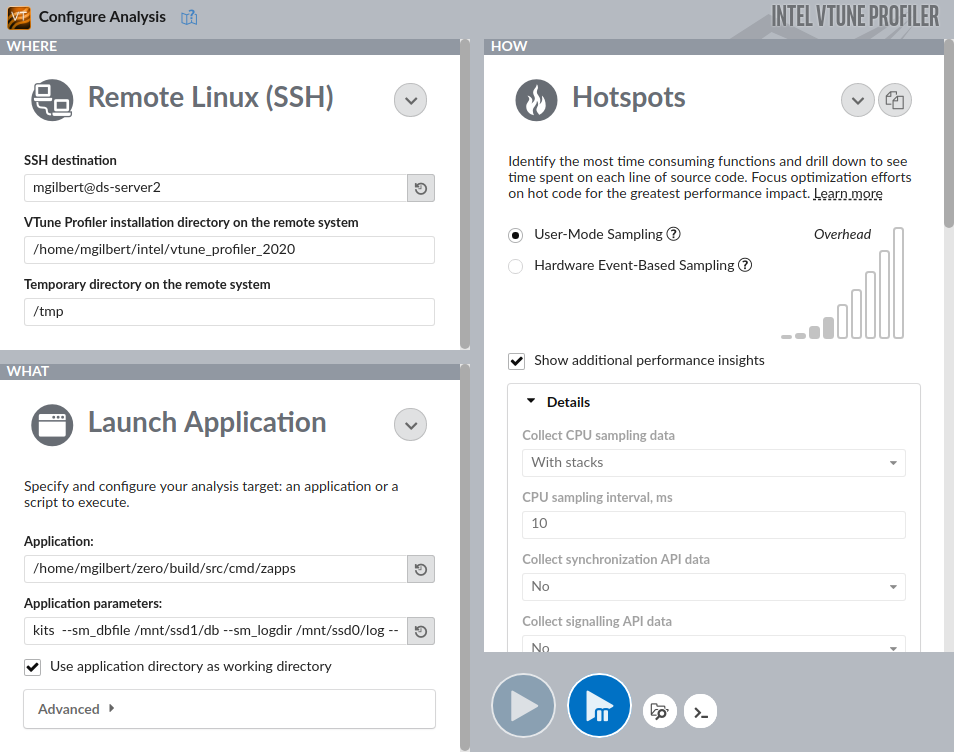
\includegraphics[width = \textwidth-2pt]{data/Intel_VTune_Profiler_Configure_Analysis.png}%
        }
        \vspace{.125em}
        \caption[Configuration of an analysis with Intel® VTune™ Profiler]{In \textit{Intel® VTune™ Profiler}, the configuration of an analysis via GUI is clearly structured: \textbf{How} should \textbf{what} software running \textbf{where} be analyzed?}
        \label{fig:vtuneconfig}
    \end{figure}
\end{@empty}

    The software allows naming of the generated analyses and their management in \emph{projects}, which makes it easier to keep track of all generated results. But these functionalities are not as comfortable as they could be---an analysis cannot be named during configuration. The results have to be generated first to give it its own name afterwards. And after renaming an analysis, the results must be reloaded by the software---resetting the analysis viewer.

    But before the first analysis can be created, a \emph{license} for the software must be acquired and the \textit{VTune™ Profiler} needs to be installed. The \emph{installation} can be done via command line or GUI. But for example, if the target software is running on a server, only the \emph{sampling driver} needs to be installed there, while it is controlled by a full \textit{VTune™ Profiler} installation on the PC on which the analyses are initiated and evaluated.

    But once the software (and the sampling driver on a potentially separate target system) is installed, the first analysis can be started. Figure \ref{fig:vtuneconfig} shows the \emph{configuration dialog} for a \textit{VTune™ Profiler} analysis via GUI. It is divided into \emph{three main topics}.

\begin{@empty}
    \setlength{\fboxsep}{0pt}%
    \setlength{\fboxrule}{1pt}%
    
    \begin{figure}[h]
        \centering
        \fbox{%
            
\includegraphics[width = .75\textwidth]{data/Intel_VTune_Profiler_Configure_Where.png}%
        }
        \vspace{.75em}
        \caption[Where is the VTune™ Profiler target running?]{The \textit{Intel® VTune™ Profiler} does not only allow the analysis of software running local.}
        \label{fig:vtunewhere}
    \end{figure}
\end{@empty}

    First, it is required to decide \textbf{where} to run the target software on---figure \ref{fig:vtuneconfig} shows the different options. For example, if ``Remote Linux (SSH)'' is selected, as in the example shown in figure \ref{fig:vtuneconfig}, the local \textit{VTune™ Profiler} will connect to the target system, where at least the \emph{sampling driver} must be installed, via \textit{SSH}, conveniently using the user's configuration for SSH connections.

\begin{@empty}
    \setlength{\fboxsep}{0pt}%
    \setlength{\fboxrule}{1pt}%
    
    \begin{figure}[h]
        \centering
        \fbox{%
            
\includegraphics[width = .75\textwidth]{data/Intel_VTune_Profiler_Configure_What.png}%
        }
        \vspace{.75em}
        \caption[What is analyzed by the VTune™ Profiler?]{The \textit{Intel® VTune™ Profiler} can also attach to an already running process to analyze that.}
        \label{fig:vtunewhat}
    \end{figure}
\end{@empty}

    The second decision to be made is the question of \textbf{what} to analyze on the target system by the \textit{VTune™ Profiler}. Figure \ref{fig:vtunewhat} shows the different options. While ``Profile System'' and ``Attach to Process'' can also be used to evaluate a production system, the ``Launch Application'' option is best suited for the measurements performed for this chapter. With this option, the target application is started by the \textit{VTune™ Profiler} and specified parameters are passed to it. Data acquisition can be delayed, and a maximum amount of data or time span for data acquisition can be specified, for example, to omit the start and shutdown procedures of the target application from analysis.

\begin{@empty}
    \setlength{\fboxsep}{0pt}%
    \setlength{\fboxrule}{1pt}%
    
    \begin{figure}[h]
        \centering
        \fbox{%
            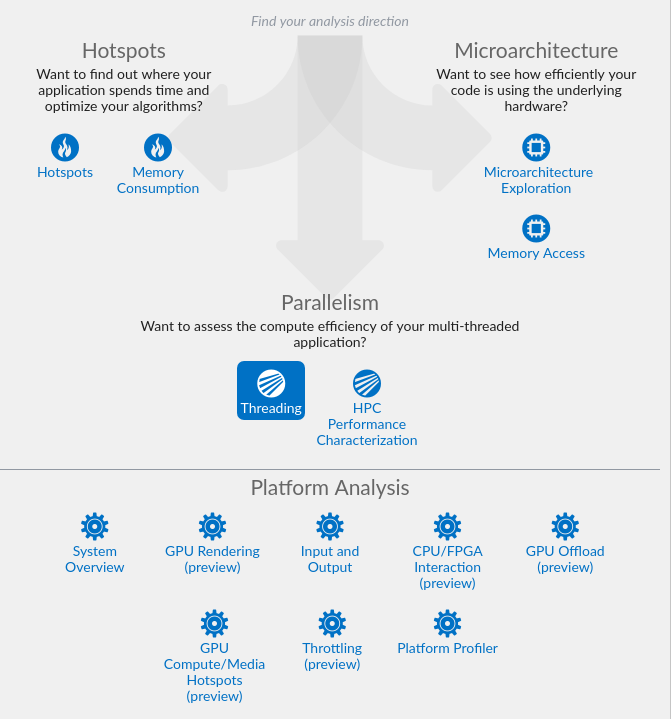
\includegraphics[width = .75\textwidth]{data/Intel_VTune_Profiler_Configure_How.png}%
        }
        \vspace{.75em}
        \caption[How should the VTune™ Profiler analyze the target?]{The \textit{Intel® VTune™ Profiler} offers a number of presets that define which events should be collected during analysis and how this data should be post-processed afterwards.}
        \label{fig:vtunehow}
    \end{figure}
\end{@empty}

    With the final decision, the user tells the \textit{VTune™ Profiler} their intention for the analysis---\textbf{how} should the \textit{VTune™ Profiler} create the analysis? The \textit{Intel® VTune™ Profiler} provides a set of \emph{presets} for various analyses---each preset defines the \emph{events to be counted} and the \emph{sample rate} for \emph{stack traces}, allowing the identification of components, functions, or code lines causing these events.

\begin{@empty}
    \setlength{\fboxsep}{0pt}%
    \setlength{\fboxrule}{1pt}%
    
    \begin{figure}[h!]
        \centering
        \fbox{%
            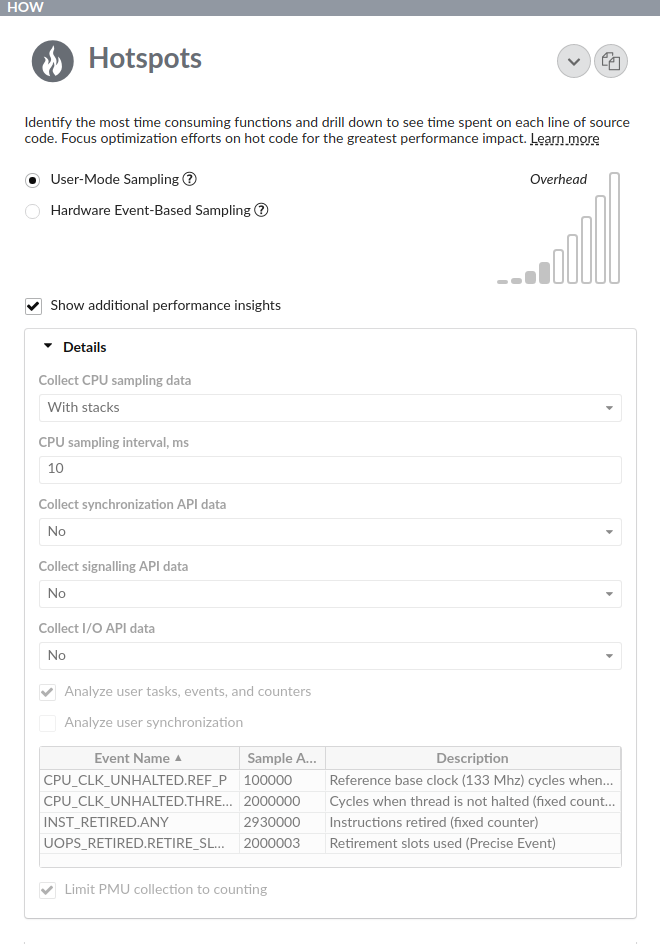
\includegraphics[width = .75\textwidth]{data/Intel_VTune_Profiler_Configure_Hotspots.png}%
        }
        \vspace{.75em}
        \caption[``Hotspots'' preset of the VTune™ Profiler]{The ``Hotspots'' preset of the \textit{Intel® VTune™ Profiler} specifies among many other options the CPU sampling interval and the events to be counted. Many less relevant options that are not used by this preset have been removed from this screenshot.}
        \label{fig:vtunehotspots}
    \end{figure}
\end{@empty}

    The preset  can be used for example with ``User-Mode Sampling'' or with ``Hardware Event-Based Sampling''. ``User-Mode Sampling'' \emph{interrupts} the analyzed process (defined in ``what'') every \SI{10}{\milli\second} (default ``CPU sampling interval'') and stores the current \emph{call stack} of each unhalted thread of the process. The CPU time since the previous sample is then assigned to that captured call stack. Afterwards, the stack trace is \emph{aggregated} by summing the CPU times of identical call stacks to obtain a---statistically exact---allocation of CPU time to different call stacks. ``Hardware Event-Based Sampling'' also interrupts the analyzed process to store the call stacks, but it assigns the values of certain \emph{hardware counters} to each sample, so that different samples contribute to the final summary based on these values. These hardware counters can count e.g. CPU cycles, executed instructions, L2 cache misses or branch mispredictions---depending on the capabilities of the CPU architecture. Figure \ref{fig:vtunehotspots} shows some settings of the ``Hotspots'' preset, but many others, e.g. regarding GPU usage and memory, have been removed from the screenshot for the sake of clarity.

\begin{@empty}
    \setlength{\fboxsep}{0pt}%
    \setlength{\fboxrule}{1pt}%
    
    \begin{figure}[h!]
        \centering
        \fbox{%
            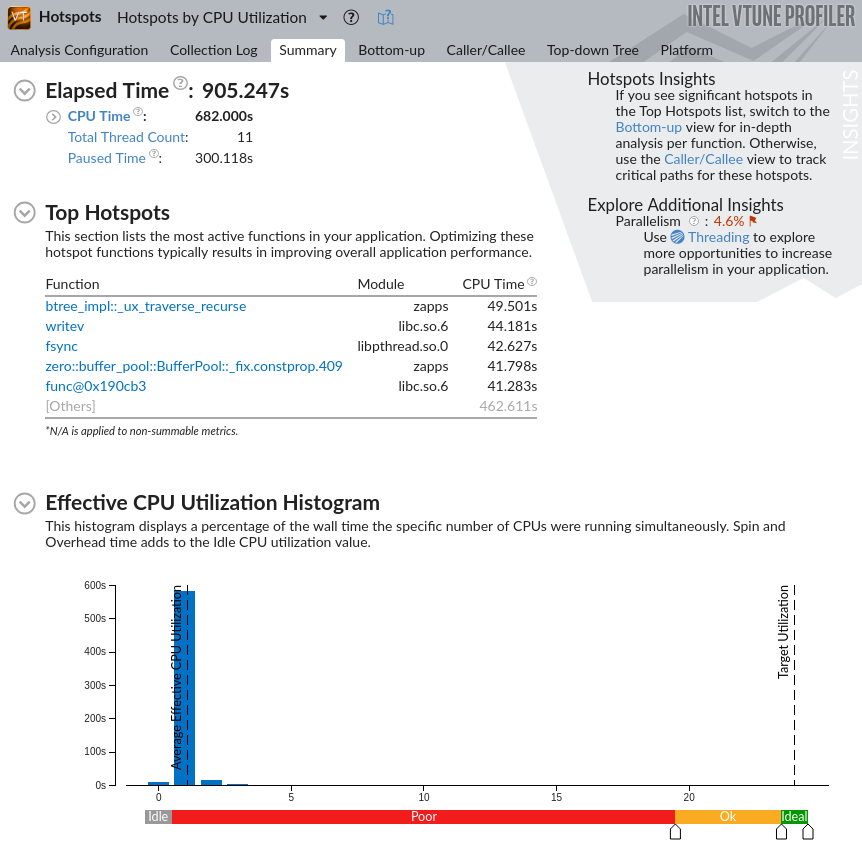
\includegraphics[width = .75\textwidth]{data/Intel_VTune_Profiler_Results_Summary.png}%
        }
        \vspace{.75em}
        \caption[Summary of an analysis done by the VTune™ Profiler]{The \textit{Intel® VTune™ Profiler} provides a ``Summary'' tab for each analysis performed, displaying---depending on configuration---highlights related to various performance aspects.}
        \label{fig:vtunesummary}
    \end{figure}
\end{@empty}

    The \textit{VTune™ Profiler} presents the results of each analysis in a variety of ways, divided among different tabs. An exemplary ``Summary'' tab of the ``Hotspots'' preset when using ``User-Mode Sampling'' is shown in figure \ref{fig:vtunesummary}. It shows a \emph{ranking of the functions} that required the most CPU time and a visualization of the \emph{degree of parallelism} achieved.

\begin{@empty}
    \setlength{\fboxsep}{0pt}%
    \setlength{\fboxrule}{1pt}%
    
    \begin{figure}[h!]
        \centering
        \fbox{%
            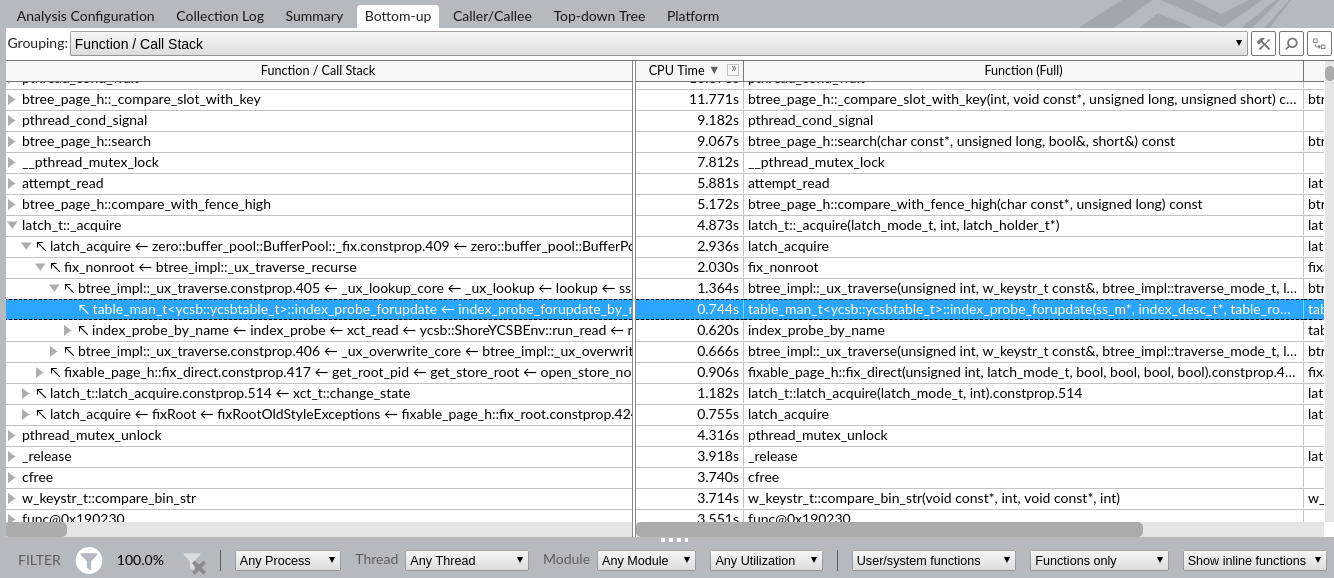
\includegraphics[width = \textwidth]{data/Intel_VTune_Profiler_Results_BottomUp.png}%
        }
        \vspace{.75em}
        \caption[Bottom-up view of an analysis done by the VTune™ Profiler]{The ``Bottom-up'' tab of a \textit{Intel® VTune™ Profiler} analysis summarizes the collected samples based on the lowest element of the call stacks.}
        \label{fig:vtunebottomup}
    \end{figure}
\end{@empty}

    The ``Bottom-up'' tab breaks down CPU time (or other performance characteristics) based on the \emph{bottom element of the call stack} of each sample. This element is the function (or loop, if displayed) that was running on the CPU at the time the sample was taken. As shown in the figure \ref{fig:vtunebottomup}, the callers (and their callers) to these functions can also be displayed along with a breakdown of the share of CPU time of each combination.

    The samples considered for the summaries in the ``Bottom-up'' tab and the other tabs can be \emph{filtered} by timestamp, process, thread and software module. These filter options are shown at the bottom of the figure \ref{fig:vtunebottomup}.

\begin{@empty}
    \setlength{\fboxsep}{0pt}%
    \setlength{\fboxrule}{1pt}%
    
    \begin{figure}[h!]
        \centering
        \fbox{%
            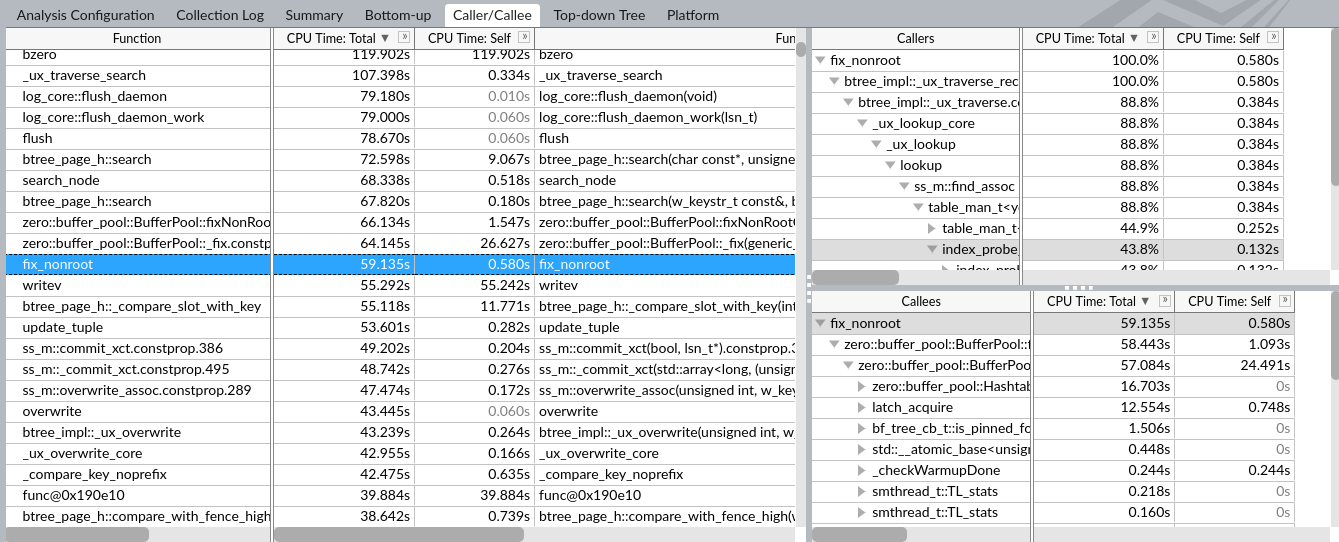
\includegraphics[width = \textwidth]{data/Intel_VTune_Profiler_Results_CallerCallee.png}%
        }
        \vspace{.75em}
        \caption[Caller/Callee view of an analysis done by the VTune™ Profiler]{The ``Caller/Callee'' tab of a \textit{Intel® VTune™ Profiler} analysis lists the total CPU time used by each function---including the called functions.}
        \label{fig:vtunecallercallee}
    \end{figure}
\end{@empty}

    The ``Caller/Callee'' tab lists \emph{each function contained in the stack trace} and assigns it the CPU time it requires including that of any functions it calls. Therefore, the entry point of the program is usually the function with the highest CPU time required---it is the base of every call and every thread spawn. This list is shown in the \emph{left frame} in figure \ref{fig:vtunecallercallee}. The callers and callees to these functions can then be retrieved as shown for \lstinline|fix_nonroot| in the example. The \emph{upper right frame} in the figure shows the callers as they are displayed in the ``Bottom-up'' tab. The callees can be displayed in the same way as they are shown in the ``Top-down Tree'' tab. This is shown in the \emph{lower right frame} in figure \ref{fig:vtunecallercallee}.

\begin{@empty}
    \setlength{\fboxsep}{0pt}%
    \setlength{\fboxrule}{1pt}%
    
    \begin{figure}[h!]
        \centering
        \fbox{%
            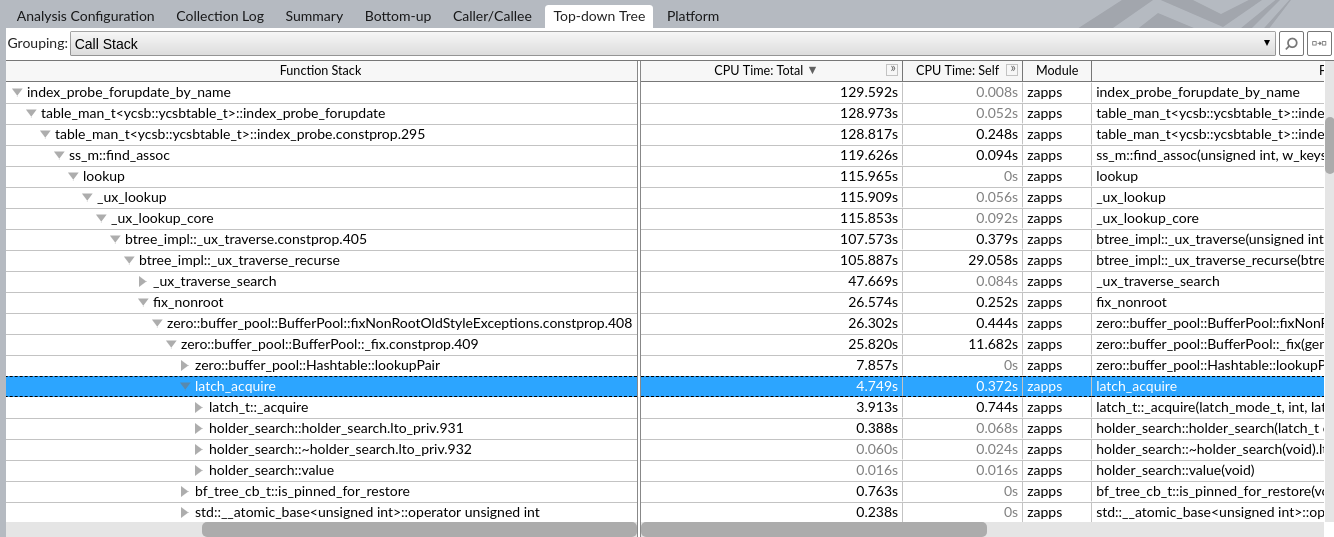
\includegraphics[width = \textwidth]{data/Intel_VTune_Profiler_Results_TopDownTree.png}%
        }
        \vspace{.75em}
        \caption[Top-down view of an analysis done by the VTune™ Profiler]{The ``Top-down Tree'' tab of a \textit{Intel® VTune™ Profiler} analysis offers the possibility to interactively discover the call stack of a program from top to bottom, sorted by e.g. CPU time.}
        \label{fig:vtunetopdowntree}
    \end{figure}
\end{@empty}

    The ``Top-down Tree'' tab initially shows only the entry point of the analyzed program and the total CPU time it has used during the analysis. From there, the view can be \emph{expanded}, as shown in figure \ref{fig:vtunetopdowntree}, to show all called functions (and the functions they call, etc.) together with the CPU time they utilize (including or excluding their callees).

\begin{@empty}
    \setlength{\fboxsep}{0pt}%
    \setlength{\fboxrule}{1pt}%
    
    \begin{figure}[h!]
        \centering
        \fbox{%
            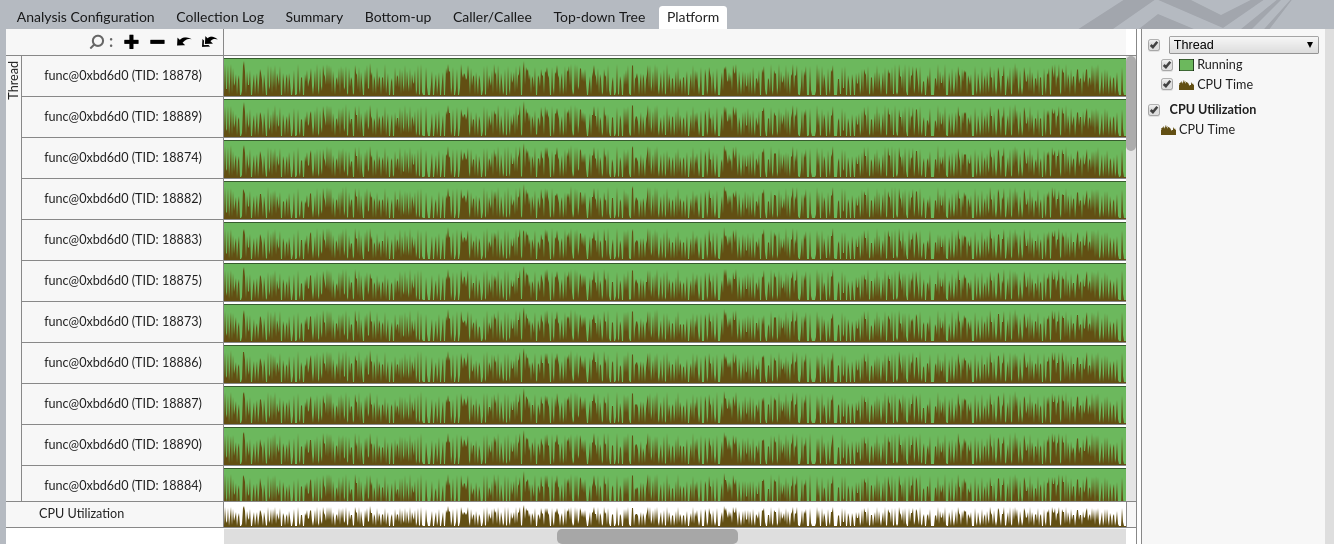
\includegraphics[width = \textwidth]{data/Intel_VTune_Profiler_Results_Platform.png}%
        }
        \vspace{.75em}
        \caption[Platform view of an analysis done by the VTune™ Profiler]{The ``Platform'' tab of a \textit{Intel® VTune™ Profiler} analysis visualizes e.g. the CPU utilization (and optionally spin time of spinlocks) per thread, process or module.}
        \label{fig:vtuneplatform}
    \end{figure}
\end{@empty}

    Finally, the ``Platform'' tab visualizes the complete analysis in terms of \emph{CPU usage}. As shown in figure \ref{fig:vtuneplatform}, it shows a graph for each thread (or alternatively process, module, or any combination of them), with CPU time displayed in brown and idle time in green. For example, if ``synchronization API data'' is collected, the spin time of spinlocks would be displayed in the graphs in red.

\subsubsection{Flaws}

    While collecting measurements for the section \ref{sec:looking_glass}, the \textit{Intel® VTune™ Profiler} showed some of its flaws.

    When ``Launch Application'' is used, it starts the target application and shows the command line output of this program during the tracing. However, this command line output is not saved together with the trace data and thus discarded when the analysis results are closed. If anything from the command line output of the analyzed program is to be used later with the analysis results---such as transaction throughput in the case of \textit{Zero}---this information must be stored outside the \textit{VTune™ Profiler}.

\section{Measurements of Harizopoulos et al. -- Redone} \label{sec:looking_glass}

    Based on the estimation that the assumptions of Harizopoulos et al. and their methodology are too restrictive, in this section their measurements are repeated with \emph{changed assumptions} and using a \emph{completely different technique}. Subsection \ref{subsec:looking_glass_methodology} describes in detail the methodology used and to demonstrate that the----probably most controversial---assumption from \cite{Harizopoulos:2008}----the unnecessity for multithreaded execution of OLTP DBS---is invalid, subsection \ref{subsec:looking_glass_single_threaded} shows the new evaluation (mostly) single-threaded while subsection \ref{subsec:looking_glass_multi_threaded} uses multithreaded execution to provide data for a comparison.

    Due to the extensive evaluation of the effect of the buffer pool size on OLTP performance in Chapter \ref{ch:page_evictioners} and the fact that today larger-than-memory databases are rarely used, \emph{only in-memory DBSs} are considered in these measurements. Since \emph{transaction support} and \emph{ACID guarantees} are still used in most OLTP applications, these are also used during the measurements. \emph{ARIES-style logging} is also used, as this is still common and built into the used prototype DBMS.

\subsection{Methodology} \label{subsec:looking_glass_methodology}

    The software used to breakdown the runtime of an OLTP system is the \emph{Intel® VTune™ Profiler 2020}, which is described in subsection \ref{subsec:vtune}. It was configured according to the outlined configuration steps as follows:

\begin{description}
    \item[Where]    The DBS was running on a ``Remote Linux (SSH)'' server. Its configuration is described in subsection \ref{subsec:page_evictioners_system_configuration}.
    \item[What]     The DBS with built-in benchmarks was started by the profiling software. Some details about the embedded DBMS used---\textit{Zero}---were given in the subsection \ref{subsec:page_evictioners_limits} and the benchmarks are \textit{TPC-C} (see subsection \ref{subsec:page_evictioners_benchmark}) and \textit{YCSB} (see subsection \ref{subsubsec:looking_glass_benchmark}). The DBS started with a clean DB (no crash recovery required), but---obviously---with an empty buffer pool. Due to the fact that a typical DBMS runs continuously---and thus with a populated buffer pool---the \textit{Intel® VTune™ Profiler} started tracing after a cold start of \SI{5}{\minute} (recording \SI{10}{\minute} total) to give realistic results.
    \item[How]      The preset ``Hotspots'' of the \textit{Intel® VTune™ Profiler} was used.
\end{description}

    The software profile generated by the \textit{Intel® VTune™ Profiler} consists of stack traces, as shown in subsection \ref{subsec:vtune}, with a total run time in seconds for each of them. Every relevant (except e.g. benchmark code such as the test data generation that would typically run on a client) stack trace is then \emph{manually assigned to one of the DBMS components} described in subsection \ref{subsubsec:looking_glass_components}. The delayed start of tracing and the overhead associated with it prevent a reliable calculation of the CPU time per transaction, so that only the percentage of CPU time used per component is shown.

\subsubsection{Benchmarks} \label{subsubsec:looking_glass_benchmark}

    The first benchmark used for the measurements in this chapter is the \emph{Yahoo! Cloud Serving Benchmark}\footnote{\url{https://ycsb.site/}} (\textit{YCSB}). It is based on a simple workload for key-value stores (\emph{NoSQL DBMSs}) and was designed for systems running in the cloud. It is for NoSQL DBMSs what \textit{TPC-C} is for OLTP SQL DBMSs.

    The DB contains \num{10000000} completely random \emph{key-value pairs} in a table with 10 character fields of \SI{100}{\byte} each mapped to a \SI{10}{\byte} key. One \emph{skewed} (based on the Zipfian distribution) random key is drawn per transaction. A read transaction reads all 10 fields associated with the key and an update transaction writes random data to a randomly selected field associated with the key. The read-only \textit{YCSB} workloads from subsection \ref{subsubsec:looking_glass_single_threaded_read_only_ycsb} and \ref{subsubsec:looking_glass_multi_threaded_read_only_ycsb} execute only read transactions, the write-only ones from subsection \ref{subsubsec:looking_glass_single_threaded_write_only_ycsb} and \ref{subsubsec:looking_glass_multi_threaded_write_only_ycsb} execute only update transactions. No transactions abort and all queried keys exist in the DB.

    The second benchmark used in this chapter---\textit{TPC-C}---performs read and (more frequently) update transactions, so that a read-write \textit{YCSB} workload is evaluated. The database and transactions of \textit{TPC-C} have already been described in the subsection \ref{subsec:page_evictioners_benchmark}.

\subsubsection{Considered DBMS Components} \label{subsubsec:looking_glass_components}

\begin{description}
    \item[B-Tree]       Each stack trace associated with maintaining the \emph{Foster B-Tree} structure or searching for keys within a B-Tree page is assigned to this component.
    \item[Logging]      The CPU time used to create log records, maintain log sequence numbers (LSNs) and flush log records to SSD is assigned to this component.
    \item[Locking]      The CPU time spent on \emph{transaction management}, acquiring and releasing locks and managing locks in the \emph{lock manager} is assigned to this component.
                        \begin{description}
                            \item[Latching] \emph{Internal structures} of transaction and lock managers require latches (not the mutexes on which the locks are based on) for synchronization in multithreaded environments. The CPU time required to acquire and release these latches is assigned to this sub-component.
                        \end{description}
    \item[Buffer Pool]  The effort for \emph{fixing and unfixing pages} is assigned to this component. In addition to the following sub-components, page eviction would also be a sub-component, but only the RANDOM page replacement algorithm and smaller-than-memory DBs are considered thus requiring no CPU time for page eviction.
                        \begin{description}
                            \item[Latching]     A latch is assigned to \emph{each buffer frame}, and a thread reading or writing a page must acquire the corresponding latch in the appropriate mode (shared or exclusive). The CPU time required to acquire and release these latches is assigned to this sub-component.
                            \item[Fetching]     Few \emph{pages are fetched from the SSD} while the stack traces are being gathered, because---due to the skewed access to the records---not all pages were accessed during the cold start phase, which is ignored by the profiler. But since the whole database fits into the buffer pool during each benchmark run, no pages need to be fetched because they were previously evicted. The CPU time required to fetch pages from the SSD is assigned to this sub-component.
                            \item[Hash Table]   The hash table \emph{maps the page identifier of each page in the buffer pool to the corresponding buffer frame index}. It is queried on each page fix---regardless of whether it is a page hit or a page miss. The runtime required to search within this hash table is assigned to this sub-component. More details about the hash table and an alternative can be found in the subsection \ref{subsec:looking_glass_swizzling}.
                            \item[Free List]    The free list is a simple concurrent \emph{queue} containing the \emph{indexes of unoccupied buffer frames}. Indexes are only dequeued when a page is fetched from SSD, so the CPU time assigned to this sub-component is very little.
                        \end{description}
\end{description}

    The \emph{logical access paths} layer, which is responsible for the mapping between internal and external records, among other things, and which is not a core component of \textit{Zero}, is not considered here. It consumes up to \SI{25}{\percent} of the CPU time, but mainly for memory operations, e.g. for creating records based on input data, so these operations would be considered \emph{useful work} by Harizopoulos et al.

\subsection{Other Related Work} \label{subsec:looking_glass_related_work}

    In contrast to Harizopoulos et al., Johnson et al. focus in \cite{Johnson:2009} on scalability in the context of multithreading. They present their successor of the \emph{Shore Storage Manager}---\textit{Shore-MT}---together with measurements to prove its better multithreading capabilities. Instead of removing modules of the \textit{Shore Storage Manager} one by one, they \emph{optimized them one after the other} and showed the increase in transaction throughput (for a simple insert-only microbenchmark) after each step. In this way, their measurements show which components of \textit{Shore Storage Manager} limit scalability to what extent.

    Pandis et al. proposed a new page latching protocol for partitioned DBSs. In their work, they compared their approach---physiological partitioning (PLP)---to the ``conventional'' approach, by breaking down the \emph{number of critical sections} per DBMS component.

    The most detailed analysis of the inner workings of a DBMS in terms of performance was conducted by Tözün et al. in \cite{Tozun:2013}. Their main goal was to compare the (micro-architectural) behavior of the OLTP benchmarks of the \emph{Transaction Processing Performance Council}---\textit{TPC-B}, \textit{TPC-C} and \textit{TPC-E}. They broke down \emph{CPU time} and \emph{other performance metrics per DBMS component} in a very similar way as here, compared CPU cache misses per cache level, and compared the behavior of the three benchmarks on systems that use \emph{Hyper-Threading Technology}.

\subsection{Single-Threaded OLTP System Analysis} \label{subsec:looking_glass_single_threaded}

    The analysis of single-threaded OLTP systems is especially relevant for the comparisons between the results of Harizopoulos et al. and the results presented here, which were obtained using a totally different methodology. However, the results can also give a better insight---compared to the results for multithreaded OLTP systems from subsection \ref{subsec:looking_glass_multi_threaded}---into the \emph{overhead of the pessimistic concurrency control}, because here---without multithreaded and interleaved execution---every operation performed by the lock manager is unnecessary.

\begin{@empty}
    \pgfplotsset{%
        every axis/.append style = {
            ylabel near ticks,
            y label style = {font = \small},
            yticklabel style = {font = \scriptsize},
            ymode = log,
            scaled y ticks = false,
            ybar = .8pt,
            xmin = -0.75,
            xmax = 2.75,
            bar width = 1.5em,
            xtick style = {draw = none},
            xtick = {0, 1, 2},
            xticklabels = {{\makecell[c]{read-only\\YCSB}}, {\makecell[c]{update-only\\YCSB}}, {\makecell[c]{\textit{TPC-C}}}},
            x tick label style = {align = center,
                                  font = \footnotesize},
            xlabel near ticks,
            x label style = {font = \small},
            ymajorgrids = true,
            legend entries = {{1 Thread}, {12 Threads}, {24 Threads}},
            legend style = {font = \footnotesize,
                            legend columns = 1,
                            /tikz/every even column/.append style = {column sep = 0.5cm}},
            width = .8\textwidth,
            height = .4\textheight
        }
    }
    
    \tikzset{%
        1thread/.style = {thick},
        12threads/.style = {thick},
        24threads/.style = {thick}
    }
    
    \nottoggle{bwmode}{
        \tikzset{%
            1thread/.append style = {draw = Cyan, fill = Cyan!25},
            12threads/.append style = {draw = Cyan, fill = Cyan!50},
            24threads/.append style = {draw = Cyan, fill = Cyan!75}
        }
    }{
        \tikzset{%
            1thread/.append style = {draw = black, fill = black!25},
            12threads/.append style = {draw = black, fill = black!50},
            24threads/.append style = {draw = black, fill = black!75}
        }
    }
    
    \begin{figure}[t]
        \centering
        \begin{tikzpicture}
            \begin{axis}[ylabel = {$\text{Transaction throughput }\left[\si{1\per\minute}\right]$},
                         legend pos = north east]
                \addplot[1thread] coordinates
                    {(0, 7313398.8) (1, 5355238.2) (2, 203286.69)};
                \addplot[12threads] coordinates
                    {(0, 16913852.4) (1, 5403291) (2, 900337.11)};
                \addplot[24threads] coordinates
                    {(0, 14604468.6) (1, 5083255.2) (2, 905283.53)};
            \end{axis}
        \end{tikzpicture}
        \caption[Transaction throughput for different thread counts]{Transaction throughput for different numbers of working threads for read/update-only \textit{YCSB} and \textit{TPC-C}}
        \label{fig:threadsthroughput}
    \end{figure}
\end{@empty}

    A quick comparison of the transaction throughput achieved with \emph{different numbers of working threads}---i.e., different numbers of threads processing transactions \emph{concurrently} and different numbers of transactions executing in an \emph{interleaved} fashion---is shown in figure \ref{fig:threadsthroughput}. The used server (see subsection \ref{subsec:page_evictioners_system_configuration}) is equipped with two CPUs, each with 6 cores, supporting 2 hardware contexts running concurrently via simultaneous multithreading, so that a total of 24 \emph{logical cores} or 12 \emph{physical cores} are available.

    The results indicate that the \emph{additional logical cores} cannot be used to increase transaction throughput. In fact, they even increase overhead through more contention and additional context switches. But \emph{read-only} \textit{YCSB} and especially \textit{TPC-C} benefit from multithreaded and interleaved transaction execution. \emph{Read-only} \textit{YCSB} can more than double its throughput if 12 instead of 1 working threads are used, \textit{TPC-C} can more than quadruple its throughput. The bottleneck of \emph{read-only} \textit{YCSB} is the contention caused by the very large number of very short transactions on a global latch in the transaction manager, which has to be acquired twice per transaction. The limited write rate of the transaction log prevents an increase in transaction throughput for \emph{update-only} \textit{YCSB}. The more balanced workload of \textit{TPC-C} can better utilize the larger number of working threads.

\subsubsection{Read-Only YCSB} \label{subsubsec:looking_glass_single_threaded_read_only_ycsb}

\begin{@empty}
    \pgfplotsset{%
        every axis/.append style = {
            ylabel = {CPU cycles $\left[\si{\percent}\right]$},
            ybar stacked,
            ylabel near ticks,
            y label style = {font = \small},
            ylabel shift = -.5em,
            ymode = normal,
            ymin = 0,
            ymax = 100,
            yticklabel style = {font = \scriptsize},
            ymode = normal,
            scaled y ticks = false,
            xmin = -0.25,
            xmax = 0.25,
            xtick = \empty,
            bar width = 0.5,
            ymajorgrids = false,
            width = .375\textwidth,
            height = .625\textheight
        }
    }

    \nottoggle{bwmode}{
        \tikzset{%
            a0/.style = {black, fill = cyan},
            a1/.style = {black, fill = cyan!80},
            a2/.style = {black, fill = cyan!60},
            a3/.style = {black, fill = cyan!40},
            a4/.style = {black, fill = cyan!20},
            b0/.style = {black, fill = magenta},
            b1/.style = {black, fill = magenta!50},
            d/.style = {black, fill = white}
        }
    }{
        \tikzset{%
            a0/.style = {black, pattern color = black!25, pattern = {Lines[angle = 45, distance = 2pt]}},
            a1/.style = {black, pattern color = black!25, pattern = {Lines[angle = 45, distance = 4pt]}},
            a2/.style = {black, pattern color = black!25, pattern = {Lines[angle = 45, distance = 6pt]}},
            a3/.style = {black, pattern color = black!25, pattern = {Lines[angle = 45, distance = 8pt]}},
            a4/.style = {black, pattern color = black!25, pattern = {Lines[angle = 45, distance = 10pt]}},
            b0/.style = {black, pattern color = black!25, pattern = {Lines[angle = -45, distance = 5pt]}},
            b1/.style = {black, pattern color = black!25, pattern = {Lines[angle = -45, distance = 10pt]}},
            d/.style = {black, fill = white}
        }
    }

    \begin{figure}[h!]
        \centering
        \begin{tikzpicture}[remember picture]
            \begin{axis}[ymax = 100]
                \node[] at ($(0, 0)!.5!(0, 8.27+0.13+4.44+4.14+5.30)$) {\makecell[c]{\contour{white}{Buffer pool}\\\footnotesize \contour{white}{\SI{22.28}{\percent}}}};
                \node[] at ($(0, 8.27+0.13+4.44+4.14+5.30)!.5!(0, 8.27+0.13+4.44+4.14+5.30+32.09+2.38)$) {\makecell[c]{\contour{white}{Locking}\\\footnotesize \contour{white}{\SI{34.47}{\percent}}}};
                \node[] at ($(0, 8.27+0.13+4.44+4.14+5.30+32.09+2.38)!.5!(0, 8.27+0.13+4.44+4.14+5.30+32.09+2.38+1.01)$) {\scriptsize\makecell[c]{\contour{white}{Logging \SI{1.01}{\percent}}}};
                \node[] at ($(0, 8.27+0.13+4.44+4.14+5.30+32.09+2.38+1.01)!.5!(0, 8.27+0.13+4.44+4.14+5.30+32.09+2.38+1.01+42.24)$) {\makecell[c]{\contour{white}{B-tree}\\\footnotesize \contour{white}{\SI{42.24}{\percent}}}};
        
                \addplot[d] coordinates          {(0, 0)};
                \addplot[a4]  coordinates       {(0, 8.27)};
                \addplot[a3]  coordinates       {(0, 0.13)};
                \addplot[a2]  coordinates       {(0, 4.44)};
                \addplot[a1]  coordinates       {(0, 4.14)};
                \addplot[a0] coordinates       {(0, 5.30)};
                \addplot[b1]  coordinates    {(0, 32.09)};
                \addplot[b0] coordinates    {(0, 2.38)};
                \addplot[a0] coordinates           {(0, 1.01)};
                \addplot[b0] coordinates        {(0, 42.24)};
        
                \coordinate (0rest)            at (0.25, 0);
                \coordinate (0bufferRest)      at (0.25, 8.27);
                \coordinate (0bufferFreeList)  at (0.25, 8.27+0.13);
                \coordinate (0bufferHashTable) at (0.25, 8.27+0.13+4.44);
                \coordinate (0bufferFetching)  at (0.25, 8.27+0.13+4.44+4.14);
                \coordinate (0bufferLatching)  at (0.25, 8.27+0.13+4.44+4.14+5.30);
                \coordinate (0lockingRest)     at (0.25, 8.27+0.13+4.44+4.14+5.30+32.09);
                \coordinate (0lockingLatching) at (0.25, 8.27+0.13+4.44+4.14+5.30+32.09+2.38);
            \end{axis}
        \end{tikzpicture}
        \hspace{4em}
        \begin{tikzpicture}[remember picture]
            \begin{axis}[ylabel = { },
                         ymax = 8.27+0.13+4.44+4.14+5.30+32.09+2.38]
                \node[] at ($(0, 8.27)!.5!(0, 8.27+0.13)$)  {\scriptsize\makecell[c]{\contour{white}{Free list \SI{0.13}{\percent}}}};
                \node[] at ($(0, 8.27+0.13)!.5!(0, 8.27+0.13+4.44)$) {\scriptsize\makecell[c]{\contour{white}{Hash table \SI{4.44}{\percent}}}};
                \node[] at ($(0, 8.27+0.13+4.44)!.5!(0, 8.27+0.13+4.44+4.14)$){\scriptsize\makecell[c]{\contour{white}{Fetching} \contour{white}{\SI{4.14}{\percent}}}};
                \node[] at ($(0, 8.27+0.13+4.44+4.14)!.5!(0, 8.27+0.13+4.44+4.14+5.30)$){\makecell[c]{\contour{white}{Latching}\\\footnotesize \contour{white}{\SI{5.3}{\percent}}}};
                \node[anchor = north, inner ysep = .5pt] at (0, 8.27+0.13+4.44+4.14+5.30+32.09+2.38){\scriptsize\makecell[c]{\contour{white}{Latching \SI{2.38}{\percent}}}};
        
                \addplot[a4]  coordinates       {(0, 8.27)};
                \addplot[a3]  coordinates       {(0, 0.13)};
                \addplot[a2]  coordinates       {(0, 4.44)};
                \addplot[a1]  coordinates       {(0, 4.14)};
                \addplot[a0] coordinates       {(0, 5.30)};
                \addplot[b1]  coordinates    {(0, 32.09)};
                \addplot[b0] coordinates    {(0, 2.38)};
        
                \coordinate (1rest)            at (-0.25, 0);
                \coordinate (1bufferRest)      at (-0.25, 8.27);
                \coordinate (1bufferFreeList)  at (-0.25, 8.27+0.13);
                \coordinate (1bufferHashTable) at (-0.25, 8.27+0.13+4.44);
                \coordinate (1bufferFetching)  at (-0.25, 8.27+0.13+4.44+4.14);
                \coordinate (1bufferLatching)  at (-0.25, 8.27+0.13+4.44+4.14+5.30);
                \coordinate (1lockingRest)     at (-0.25, 8.27+0.13+4.44+4.14+5.30+32.09);
                \coordinate (1lockingLatching) at (-0.25, 8.27+0.13+4.44+4.14+5.30+32.09+2.38);
            \end{axis}
        \end{tikzpicture}
        \begin{tikzpicture}[remember picture,
                            overlay]
            \draw (0rest)[draw = black]            -- (1rest);
            \draw (0bufferRest)[draw = black]      -- (1bufferRest);
            \draw (0bufferFreeList)[draw = black]  -- (1bufferFreeList);
            \draw (0bufferHashTable)[draw = black] -- (1bufferHashTable);
            \draw (0bufferFetching)[draw = black]  -- (1bufferFetching);
            \draw (0bufferLatching)[draw = black]  -- (1bufferLatching);
            \draw (0lockingRest)[draw = black]     -- (1lockingRest);
            \draw (0lockingLatching)[draw = black] -- (1lockingLatching);
        \end{tikzpicture}
        \caption[CPU cycles breakdown for single-threaded read-only YCSB]{Component-wise breakdown of the CPU cycles when running read-only \textit{YCSB} with one querying terminal.}
        \label{fig:cyclesycsbread1}
    \end{figure}
\end{@empty}

    Figure \ref{fig:cyclesycsbread1} shows the breakdown of CPU time of \textit{Zero} when running \emph{read-only} \textit{YCSB} on 1 working thread and a DB smaller than the buffer pool. While this diagram only shows the percentage of CPU time per DBMS component, CPU times in seconds are given in table \ref{tab:breakdown} later in this section.

    Since \emph{read-only} workloads do not generate log entries, \emph{logging} here only accounts for \SI{1.01}{\percent} of the total CPU time. The only overhead of the transaction log is caused by the need to store the current LSN for each transaction at the time it begins.

    The \SI{4.14}{\percent} of CPU time used to \emph{fetch pages} from the SSD (and the \SI{0.13}{\percent} used to access the buffer pool's free list) is \emph{caused by the skewed DB accesses} of \textit{YCSB} where not all pages used during the benchmark run were referenced during the buffer pool warmup.

    Because of the very large number of simple transactions that are being executed, the lock manager and mainly the \emph{transaction manager} use \SI{34.47}{\percent} of CPU time. This overhead is caused by management tasks required whenever a transaction begins or commits.

    During single-threaded execution, no concurrency control is required, so \emph{lock management} and \emph{buffer frame latching}---which accounts for \SI{5.3}{\percent} of CPU time---are a waste of resources.

\subsubsection{Write-Only YCSB} \label{subsubsec:looking_glass_single_threaded_write_only_ycsb}

\begin{@empty}
    \pgfplotsset{%
        every axis/.append style = {
            ylabel = {CPU cycles $\left[\si{\percent}\right]$},
            ybar stacked,
            ylabel near ticks,
            y label style = {font = \small},
            ylabel shift = -.5em,
            ymode = normal,
            ymin = 0,
            ymax = 100,
            yticklabel style = {font = \scriptsize},
            ymode = normal,
            scaled y ticks = false,
            xmin = -0.25,
            xmax = 0.25,
            xtick = \empty,
            bar width = 0.5,
            ymajorgrids = false,
            width = .375\textwidth,
            height = .625\textheight
        }
    }

    \nottoggle{bwmode}{
        \tikzset{%
            a0/.style = {black, fill = cyan},
            a1/.style = {black, fill = cyan!80},
            a2/.style = {black, fill = cyan!60},
            a3/.style = {black, fill = cyan!40},
            a4/.style = {black, fill = cyan!20},
            b0/.style = {black, fill = magenta},
            b1/.style = {black, fill = magenta!50},
            d/.style = {black, fill = white}
        }
    }{
        \tikzset{%
            a0/.style = {black, pattern color = black!25, pattern = {Lines[angle = 45, distance = 2pt]}},
            a1/.style = {black, pattern color = black!25, pattern = {Lines[angle = 45, distance = 4pt]}},
            a2/.style = {black, pattern color = black!25, pattern = {Lines[angle = 45, distance = 6pt]}},
            a3/.style = {black, pattern color = black!25, pattern = {Lines[angle = 45, distance = 8pt]}},
            a4/.style = {black, pattern color = black!25, pattern = {Lines[angle = 45, distance = 10pt]}},
            b0/.style = {black, pattern color = black!25, pattern = {Lines[angle = -45, distance = 5pt]}},
            b1/.style = {black, pattern color = black!25, pattern = {Lines[angle = -45, distance = 10pt]}},
            d/.style = {black, fill = white}
        }
    }
    
    \begin{figure}[h!]
        \centering
        \begin{tikzpicture}[remember picture]
            \begin{axis}[ymax = 100]
                \node[] at ($(0, 0)!.5!(0, 6.17+0.07+3.46+1.17+5.17)$) {\makecell[c]{\contour{white}{Buffer pool}\\\footnotesize \contour{white}{\SI{16.04}{\percent}}}};
                \node[] at ($(0, 6.17+0.07+3.46+1.17+5.17)!.5!(0, 6.17+0.07+3.46+1.17+5.17+19.19+2.54)$) {\makecell[c]{\contour{white}{Locking}\\\footnotesize \contour{white}{\SI{21.73}{\percent}}}};
                \node[] at ($(0, 6.17+0.07+3.46+1.17+5.17+19.19+2.54)!.5!(0, 6.17+0.07+3.46+1.17+5.17+19.19+2.54+24.42)$) {\makecell[c]{\contour{white}{Logging}\\\footnotesize \contour{white}{\SI{24.42}{\percent}}}};
                \node[] at ($(0, 6.17+0.07+3.46+1.17+5.17+19.19+2.54+24.42)!.5!(0, 6.17+0.07+3.46+1.17+5.17+19.19+2.54+24.42+37.81)$) {\makecell[c]{\contour{white}{B-tree}\\\footnotesize \contour{white}{\SI{37.81}{\percent}}}};
        
                \addplot[d] coordinates          {(0, 0)};
                \addplot[a4]  coordinates       {(0, 6.17)};
                \addplot[a3]  coordinates       {(0, 0.07)};
                \addplot[a2]  coordinates       {(0, 3.46)};
                \addplot[a1]  coordinates       {(0, 1.17)};
                \addplot[a0] coordinates       {(0, 5.17)};
                \addplot[b1]  coordinates    {(0, 19.19)};
                \addplot[b0] coordinates    {(0, 2.54)};
                \addplot[a0] coordinates           {(0, 24.42)};
                \addplot[b0] coordinates        {(0, 37.81)};
        
                \coordinate (0rest)            at (0.25, 0);
                \coordinate (0bufferRest)      at (0.25, 6.17);
                \coordinate (0bufferFreeList)  at (0.25, 6.17+0.07);
                \coordinate (0bufferHashTable) at (0.25, 6.17+0.07+3.46);
                \coordinate (0bufferFetching)  at (0.25, 6.17+0.07+3.46+1.17);
                \coordinate (0bufferLatching)  at (0.25, 6.17+0.07+3.46+1.17+5.17);
                \coordinate (0lockingRest)     at (0.25, 6.17+0.07+3.46+1.17+5.17+19.19);
                \coordinate (0lockingLatching) at (0.25, 6.17+0.07+3.46+1.17+5.17+19.19+2.54);
            \end{axis}
        \end{tikzpicture}
        \hspace{4em}
        \begin{tikzpicture}[remember picture]
            \begin{axis}[ylabel = { },
                         ymax = 6.17+0.07+3.46+1.17+5.17+19.19+2.54]
                \node[] at ($(0, 6.17)!.5!(0, 6.17+0.07)$)  {\scriptsize\makecell[c]{\contour{white}{Free list \SI{0.07}{\percent}}}};
                \node[] at ($(0, 6.17+0.07)!.5!(0, 6.17+0.07+3.46)$) {\scriptsize\makecell[c]{\contour{white}{Hash table \SI{3.46}{\percent}}}};
                \node[] at ($(0, 6.17+0.07+3.46)!.5!(0, 6.17+0.07+3.46+1.17)$){\scriptsize\makecell[c]{\contour{white}{Fetching} \contour{white}{\SI{1.17}{\percent}}}};
                \node[] at ($(0, 6.17+0.07+3.46+1.17)!.5!(0, 6.17+0.07+3.46+1.17+5.17)$){\makecell[c]{\contour{white}{Latching}\\\footnotesize \contour{white}{\SI{5.17}{\percent}}}};
                \node[] at ($(0, 6.17+0.07+3.46+1.17+5.17+19.19)!.5!(0, 6.17+0.07+3.46+1.17+5.17+19.19+2.54)$){\scriptsize\makecell[c]{\contour{white}{Latching \SI{2.54}{\percent}}}};
        
                \addplot[a4]  coordinates       {(0, 6.17)};
                \addplot[a3]  coordinates       {(0, 0.07)};
                \addplot[a2]  coordinates       {(0, 3.46)};
                \addplot[a1]  coordinates       {(0, 1.17)};
                \addplot[a0] coordinates       {(0, 5.17)};
                \addplot[b1]  coordinates    {(0, 19.19)};
                \addplot[b0] coordinates    {(0, 2.54)};
        
                \coordinate (1rest)            at (-0.25, 0);
                \coordinate (1bufferRest)      at (-0.25, 6.17);
                \coordinate (1bufferFreeList)  at (-0.25, 6.17+0.07);
                \coordinate (1bufferHashTable) at (-0.25, 6.17+0.07+3.46);
                \coordinate (1bufferFetching)  at (-0.25, 6.17+0.07+3.46+1.17);
                \coordinate (1bufferLatching)  at (-0.25, 6.17+0.07+3.46+1.17+5.17);
                \coordinate (1lockingRest)     at (-0.25, 6.17+0.07+3.46+1.17+5.17+19.19);
                \coordinate (1lockingLatching) at (-0.25, 6.17+0.07+3.46+1.17+5.17+19.19+2.54);
            \end{axis}
        \end{tikzpicture}
        \begin{tikzpicture}[remember picture,
                            overlay]
            \draw (0rest)[draw = black]            -- (1rest);
            \draw (0bufferRest)[draw = black]      -- (1bufferRest);
            \draw (0bufferFreeList)[draw = black]  -- (1bufferFreeList);
            \draw (0bufferHashTable)[draw = black] -- (1bufferHashTable);
            \draw (0bufferFetching)[draw = black]  -- (1bufferFetching);
            \draw (0bufferLatching)[draw = black]  -- (1bufferLatching);
            \draw (0lockingRest)[draw = black]     -- (1lockingRest);
            \draw (0lockingLatching)[draw = black] -- (1lockingLatching);
        \end{tikzpicture}
        \caption[CPU cycles breakdown for single-threaded update-only YCSB]{Component-wise breakdown of the CPU cycles when running update-only \textit{YCSB} with one querying terminal.}
        \label{fig:cyclesycsbwrite1}
    \end{figure}
\end{@empty}

    Figure \ref{fig:cyclesycsbwrite1} shows the CPU time breakdown of \textit{Zero} when running \emph{update-only} \textit{YCSB} on 1 working thread and a DB smaller than the buffer pool.

    Just like the \emph{read-only} \textit{YCSB}, the \emph{update-only} \textit{YCSB} does not access all used DB pages during buffer pool warmup. However, due to the lower transaction throughput of this workload, significantly fewer pages have to be \emph{fetched} using only $\SI{1.17}{\percent} + \SI{0.07}{\percent}$ of the total CPU time.

    In contrast to \emph{read-only} workloads, each transaction of the \emph{update-only} \textit{YCSB} results in the creation and writing of a log entry, which results in \SI{24.42}{\percent} of the CPU time used for \emph{logging}.

    The just a little smaller number of simple transactions executed with the \emph{update-only} variant causes the \emph{lock and transaction managers} to use \SI{21.73}{\percent} of CPU time. As can be seen in table \ref{tab:breakdown}, the absolute CPU time used by these components reflects what is expected taking into account the transaction throughput and CPU time required during read-only \textit{YCSB}.

    The lower transaction throughput does not reduce the absolute CPU time used by the \emph{Foster B-tree}, although fewer records are accessed. The lower overhead imposed by the \emph{buffer pool}---compared to the measurement with \emph{read-only} \textit{YCSB}---is similar to what would be expected considering the lower transaction throughput.

\subsubsection{TPC-C} \label{subsubsec:looking_glass_single_threaded_tpcc}

\begin{@empty}
    \pgfplotsset{%
        every axis/.append style = {
            ylabel = {CPU cycles $\left[\si{\percent}\right]$},
            ybar stacked,
            ylabel near ticks,
            y label style = {font = \small},
            ylabel shift = -.5em,
            ymode = normal,
            ymin = 0,
            ymax = 100,
            yticklabel style = {font = \scriptsize},
            ymode = normal,
            scaled y ticks = false,
            xmin = -0.25,
            xmax = 0.25,
            xtick = \empty,
            bar width = 0.5,
            ymajorgrids = false,
            width = .375\textwidth,
            height = .625\textheight
        }
    }

    \nottoggle{bwmode}{
        \tikzset{%
            a0/.style = {black, fill = cyan},
            a1/.style = {black, fill = cyan!80},
            a2/.style = {black, fill = cyan!60},
            a3/.style = {black, fill = cyan!40},
            a4/.style = {black, fill = cyan!20},
            b0/.style = {black, fill = magenta},
            b1/.style = {black, fill = magenta!50},
            d/.style = {black, fill = white}
        }
    }{
        \tikzset{%
            a0/.style = {black, pattern color = black!25, pattern = {Lines[angle = 45, distance = 2pt]}},
            a1/.style = {black, pattern color = black!25, pattern = {Lines[angle = 45, distance = 4pt]}},
            a2/.style = {black, pattern color = black!25, pattern = {Lines[angle = 45, distance = 6pt]}},
            a3/.style = {black, pattern color = black!25, pattern = {Lines[angle = 45, distance = 8pt]}},
            a4/.style = {black, pattern color = black!25, pattern = {Lines[angle = 45, distance = 10pt]}},
            b0/.style = {black, pattern color = black!25, pattern = {Lines[angle = -45, distance = 5pt]}},
            b1/.style = {black, pattern color = black!25, pattern = {Lines[angle = -45, distance = 10pt]}},
            d/.style = {black, fill = white}
        }
    }
    
    \begin{figure}[h!]
        \centering
        \begin{tikzpicture}[remember picture]
            \begin{axis}[ymax = 100]
                \node[] at ($(0, 0)!.5!(0, 8.84+0.05+4.56+0.49+6.17)$) {\makecell[c]{\contour{white}{Buffer pool}\\\footnotesize \contour{white}{\SI{20.11}{\percent}}}};
                \node[] at ($(0, 8.84+0.05+4.56+0.49+6.17)!.5!(0, 8.84+0.05+4.56+0.49+6.17+4.55+0.36)$) {\scriptsize\makecell[c]{\contour{white}{Locking \SI{4.91}{\percent}}}};
                \node[] at ($(0, 8.84+0.05+4.56+0.49+6.17+4.55+0.36)!.5!(0, 8.84+0.05+4.56+0.49+6.17+4.55+0.36+42.46)$) {\makecell[c]{\contour{white}{Logging}\\\footnotesize \contour{white}{\SI{42.46}{\percent}}}};
                \node[] at ($(0, 8.84+0.05+4.56+0.49+6.17+4.55+0.36+42.46)!.5!(0, 8.84+0.05+4.56+0.49+6.17+4.55+0.36+42.46+32.51)$) {\makecell[c]{\contour{white}{B-tree}\\\footnotesize \contour{white}{\SI{32.51}{\percent}}}};

                \addplot[d] coordinates          {(0, 0)};
                \addplot[a4]  coordinates       {(0, 8.84)};
                \addplot[a3]  coordinates       {(0, 0.05)};
                \addplot[a2]  coordinates       {(0, 4.56)};
                \addplot[a1]  coordinates       {(0, 0.49)};
                \addplot[a0] coordinates       {(0, 6.17)};
                \addplot[b1]  coordinates    {(0, 4.55)};
                \addplot[b0] coordinates    {(0, 0.36)};
                \addplot[a0] coordinates           {(0, 42.46)};
                \addplot[b0] coordinates        {(0, 32.51)};

                \coordinate (0rest)            at (0.25, 0);
                \coordinate (0bufferRest)      at (0.25, 8.84);
                \coordinate (0bufferFreeList)  at (0.25, 8.84+0.05);
                \coordinate (0bufferHashTable) at (0.25, 8.84+0.05+4.56);
                \coordinate (0bufferFetching)  at (0.25, 8.84+0.05+4.56+0.49);
                \coordinate (0bufferLatching)  at (0.25, 8.84+0.05+4.56+0.49+6.17);
                \coordinate (0lockingRest)     at (0.25, 8.84+0.05+4.56+0.49+6.17+4.55);
                \coordinate (0lockingLatching) at (0.25, 8.84+0.05+4.56+0.49+6.17+4.55+0.36);
            \end{axis}
        \end{tikzpicture}
        \hspace{4em}
        \begin{tikzpicture}[remember picture]
            \begin{axis}[ylabel = { },
                         ymax = 8.84+0.05+4.56+0.49+6.17+4.55+0.36]
                \node[] at ($(0, 8.84)!.5!(0, 8.84+0.05)$)  {\scriptsize\makecell[c]{\contour{white}{Free list \SI{0.05}{\percent}}}};
                \node[] at ($(0, 8.84+0.05)!.5!(0, 8.84+0.05+4.56)$) {\makecell[c]{\contour{white}{Hash table}\\\footnotesize \contour{white}{\SI{4.56}{\percent}}}};
                \node[] at ($(0, 8.84+0.05+4.56)!.5!(0, 8.84+0.05+4.56+0.49)$){\scriptsize\makecell[c]{\contour{white}{Fetching} \contour{white}{\SI{0.49}{\percent}}}};
                \node[] at ($(0, 8.84+0.05+4.56+0.49)!.5!(0, 8.84+0.05+4.56+0.49+6.17)$){\makecell[c]{\contour{white}{Latching}\\\footnotesize \contour{white}{\SI{6.17}{\percent}}}};
                \node[anchor = north, inner ysep = .5pt] at (0, 8.84+0.05+4.56+0.49+6.17+4.55+0.36){\scriptsize\makecell[c]{\contour{white}{Latching \SI{0.36}{\percent}}}};

                \addplot[a4]  coordinates       {(0, 8.84)};
                \addplot[a3]  coordinates       {(0, 0.05)};
                \addplot[a2]  coordinates       {(0, 4.56)};
                \addplot[a1]  coordinates       {(0, 0.49)};
                \addplot[a0] coordinates       {(0, 6.17)};
                \addplot[b1]  coordinates    {(0, 4.55)};
                \addplot[b0] coordinates    {(0, 0.36)};

                \coordinate (1rest)            at (-0.25, 0);
                \coordinate (1bufferRest)      at (-0.25, 8.84);
                \coordinate (1bufferFreeList)  at (-0.25, 8.84+0.05);
                \coordinate (1bufferHashTable) at (-0.25, 8.84+0.05+4.56);
                \coordinate (1bufferFetching)  at (-0.25, 8.84+0.05+4.56+0.49);
                \coordinate (1bufferLatching)  at (-0.25, 8.84+0.05+4.56+0.49+6.17);
                \coordinate (1lockingRest)     at (-0.25, 8.84+0.05+4.56+0.49+6.17+4.55);
                \coordinate (1lockingLatching) at (-0.25, 8.84+0.05+4.56+0.49+6.17+4.55+0.36);
            \end{axis}
        \end{tikzpicture}
        \begin{tikzpicture}[remember picture,
                            overlay]
            \draw (0rest)[draw = black]            -- (1rest);
            \draw (0bufferRest)[draw = black]      -- (1bufferRest);
            \draw (0bufferFreeList)[draw = black]  -- (1bufferFreeList);
            \draw (0bufferHashTable)[draw = black] -- (1bufferHashTable);
            \draw (0bufferFetching)[draw = black]  -- (1bufferFetching);
            \draw (0bufferLatching)[draw = black]  -- (1bufferLatching);
            \draw (0lockingRest)[draw = black]     -- (1lockingRest);
            \draw (0lockingLatching)[draw = black] -- (1lockingLatching);
        \end{tikzpicture}
        \caption[CPU cycles breakdown for single-threaded TPC-C]{Component-wise breakdown of the CPU cycles when running \textit{TPC-C} with one querying terminal.}
        \label{fig:cyclestpcc1}
    \end{figure}
\end{@empty}

    Figure \ref{fig:cyclestpcc1} shows the breakdown of CPU time of \textit{Zero} when running \textit{TPC-C} with one working thread and a DB not growing beyond the size of the buffer pool. 

    The \textit{TPC-C} benchmark is not much less write-intensive than \emph{update-only} \textit{YCSB}. In addition to the updates performed by \textit{YCSB}, \textit{TPC-C} also inserts many records, resulting in a much larger \emph{logging} overhead of \SI{42.46}{\percent} of the total CPU time. This is twice as high a share as that measured by Harizopoulos et al. for the NEW ORDER transaction. This means that either the PAYMENT transaction---the other update transaction executed here---causes much more \emph{logging} overhead or that the log manager of \textit{Zero} is much less optimized compared to the other components of the DBMS.

    The fewer transactions that are executed, the less CPU time is used by the transaction management. Correspondingly, overhead of \emph{lock and transaction management} is just at \SI{4.91}{\percent}.

    \textit{TPC-C} fixes more pages---compared to \textit{YCSB}---containing records from several smaller \emph{B-trees} which results in fewer executed B-tree instructions (\SI{32.51}{\percent} of CPU time) and more \emph{buffer pool} work (\SI{20.11}{\percent} of CPU time).

    Harizopoulos et al. measured a much higher \emph{concurrency control} overhead and also a higher \emph{buffer pool} overhead, but much less overhead in the \emph{B-tree}. The different results for the B-tree can be explained mainly through the different approaches---the total CPU time used by the B-tree is given here, while they measured only the benefit obtained with a small optimization. But especially the \emph{lock management and latching} seems to be more optimized in \textit{Zero} compared to its predecessor, the \textit{Shore Storage Manager}.

\begin{@empty}
    \pgfplotsset{%
        every axis/.append style = {
            ylabel = {CPU cycles $\left[\si{\percent}\right]$},
            ybar stacked,
            ylabel near ticks,
            y label style = {font = \small},
            ylabel shift = -.5em,
            ymode = normal,
            ymin = 0,
            ymax = 100,
            yticklabel style = {font = \scriptsize},
            ymode = normal,
            scaled y ticks = false,
            xmin = -0.25,
            xmax = 0.25,
            xtick = \empty,
            bar width = 0.5,
            ymajorgrids = false,
            width = .375\textwidth,
            height = .625\textheight
        }
    }

    \nottoggle{bwmode}{
        \tikzset{%
            a0/.style = {black, fill = cyan},
            a1/.style = {black, fill = cyan!80},
            a2/.style = {black, fill = cyan!60},
            a3/.style = {black, fill = cyan!40},
            a4/.style = {black, fill = cyan!20},
            b0/.style = {black, fill = magenta},
            b1/.style = {black, fill = magenta!50},
            d/.style = {black, fill = white}
        }
    }{
        \tikzset{%
            a0/.style = {black, pattern color = black!25, pattern = {Lines[angle = 45, distance = 2pt]}},
            a1/.style = {black, pattern color = black!25, pattern = {Lines[angle = 45, distance = 4pt]}},
            a2/.style = {black, pattern color = black!25, pattern = {Lines[angle = 45, distance = 6pt]}},
            a3/.style = {black, pattern color = black!25, pattern = {Lines[angle = 45, distance = 8pt]}},
            a4/.style = {black, pattern color = black!25, pattern = {Lines[angle = 45, distance = 10pt]}},
            b0/.style = {black, pattern color = black!25, pattern = {Lines[angle = -45, distance = 5pt]}},
            b1/.style = {black, pattern color = black!25, pattern = {Lines[angle = -45, distance = 10pt]}},
            d/.style = {black, fill = white}
        }
    }

    \begin{figure}[h!]
        \centering
        \begin{tikzpicture}[remember picture]
            \begin{axis}[ymax = 100]
                \node[] at ($(0, 0)!.5!(0, 2.31+0.06+1.08+0.00+1.83)$) {\scriptsize\makecell[c]{\contour{white}{Buffer pool \SI{5.28}{\percent}}}};
                \node[] at ($(0, 2.31+0.06+1.08+0.00+1.83)!.5!(0, 2.31+0.06+1.08+0.00+1.83+27.65+49.94)$) {\makecell[c]{\contour{white}{Locking}\\\footnotesize \contour{white}{\SI{77.59}{\percent}}}};
                \node[] at ($(0, 2.31+0.06+1.08+0.00+1.83+27.65+49.94)!.5!(0, 2.31+0.06+1.08+0.00+1.83+27.65+49.94+0.36)$){\scriptsize\makecell[c]{\contour{white}{Logging \SI{0.36}{\percent}}}};
                \node[] at ($(0, 2.31+0.06+1.08+0.00+1.83+27.65+49.94+0.36)!.5!(0, 2.31+0.06+1.08+0.00+1.83+27.65+49.94+0.36+16.77)$){\makecell[c]{\contour{white}{B-tree}\\\footnotesize \contour{white}{\SI{16.77}{\percent}}}};
        
                \addplot[d] coordinates          {(0, 0)};
                \addplot[a4]  coordinates       {(0, 2.31)};
                \addplot[a3]  coordinates       {(0, 0.06)};
                \addplot[a2]  coordinates       {(0, 1.08)};
                \addplot[a0] coordinates       {(0, 1.83)};
                \addplot[b1]  coordinates    {(0, 27.65)};
                \addplot[b0] coordinates    {(0, 49.94)};
                \addplot[a0] coordinates           {(0, 0.36)};
                \addplot[b0] coordinates        {(0, 16.77)};
        
                \coordinate (0rest)            at (0.25, 0);
                \coordinate (0bufferRest)      at (0.25, 2.31);
                \coordinate (0bufferFreeList)  at (0.25, 2.31+0.06);
                \coordinate (0bufferHashTable) at (0.25, 2.31+0.06+1.08);
                \coordinate (0bufferFetching)  at (0.25, 2.31+0.06+1.08+0.00);
                \coordinate (0bufferLatching)  at (0.25, 2.31+0.06+1.08+0.00+1.83);
                \coordinate (0lockingRest)     at (0.25, 2.31+0.06+1.08+0.00+1.83+27.65);
                \coordinate (0lockingLatching) at (0.25, 2.31+0.06+1.08+0.00+1.83+27.65+49.94);
            \end{axis}
        \end{tikzpicture}
        \hspace{4em}
        \begin{tikzpicture}[remember picture]
            \begin{axis}[ylabel = { },
                         ymax = 2.31+0.06+1.08+0.00+1.83+27.65+49.94]
                \node[] at ($(0, 2.31)!.5!(0, 2.31+0.06)$){\scriptsize\makecell[c]{\contour{white}{Free list \SI{0.06}{\percent}}}};
                \node[] at ([yshift = .75em]$(0, 2.31)!.5!(0, 2.31+0.06)$) {\scriptsize\makecell[c]{\contour{white}{Hash table \SI{1.08}{\percent}}}};
                \node[] at ([yshift = 1.5em]$(0, 2.31)!.5!(0, 2.31+0.06)$){\scriptsize\makecell[c]{\contour{white}{Latching \SI{1.83}{\percent}}}};
                \node[] at ($(0, 2.31+0.06+1.08+0.00+1.83+27.65)!.5!(0, 2.31+0.06+1.08+0.00+1.83+27.65+49.94)$){\makecell[c]{\contour{white}{Latching}\\\footnotesize\contour{white}{\SI{49.94}{\percent}}}};

                \addplot[a4]  coordinates       {(0, 2.31)};
                \addplot[a3]  coordinates       {(0, 0.06)};
                \addplot[a2]  coordinates       {(0, 1.08)};
                \addplot[a0] coordinates       {(0, 1.83)};
                \addplot[b1]  coordinates    {(0, 27.65)};
                \addplot[b0] coordinates    {(0, 49.94)};

                \coordinate (1rest)            at (-0.25, 0);
                \coordinate (1bufferRest)      at (-0.25, 2.31);
                \coordinate (1bufferFreeList)  at (-0.25, 2.31+0.06);
                \coordinate (1bufferHashTable) at (-0.25, 2.31+0.06+1.08);
                \coordinate (1bufferFetching)  at (-0.25, 2.31+0.06+1.08+0.00);
                \coordinate (1bufferLatching)  at (-0.25, 2.31+0.06+1.08+0.00+1.83);
                \coordinate (1lockingRest)     at (-0.25, 2.31+0.06+1.08+0.00+1.83+27.65);
                \coordinate (1lockingLatching) at (-0.25, 2.31+0.06+1.08+0.00+1.83+27.65+49.94);
            \end{axis}
        \end{tikzpicture}

%        \begin{tikzpicture}[remember picture]
%            \begin{axis}[ylabel = { },
%                         ymax = (2.31+0.06+1.08+0.00+1.83+27.65+49.94)*0.125,
%                         height = .325\textheight]
%                \node[] at ($(0, 2.31)!.5!(0, 2.31+0.06)$)  {\scriptsize\makecell[c]{\contour{white}{Free list \SI{0.06}{\percent}}}};
%                \node[] at ([yshift = .75em]$(0, 2.31)!.5!(0, 2.31+0.06)$) {\scriptsize\makecell[c]{\contour{white}{Hash table \SI{1.08}{\percent}}}};
%                \node[] at ($(0, 2.31+0.06+1.08+0.00)!.5!(0, 2.31+0.06+1.08+0.00+1.83)$){\scriptsize\makecell[c]{\contour{white}{Latching \SI{1.83}{\percent}}}};
%                \node[anchor = north, inner ysep = .5pt] at (0, 2.31+0.06+1.08+0.00+1.83+27.65+49.94){\scriptsize\makecell[c]{\contour{white}{Latching \SI{49.94}{\percent}}}};
%        
%                \addplot[a4]  coordinates       {(0, 2.31)};
%                \addplot[a3]  coordinates       {(0, 0.06)};
%                \addplot[a2]  coordinates       {(0, 1.08)};
%                \addplot[a0] coordinates       {(0, 1.83)};
%                \addplot[b1]  coordinates    {(0, 27.65)};
%                \addplot[b0] coordinates    {(0, 49.94)};
%        
%                \coordinate (1rest)            at (-0.25, 0);
%                \coordinate (1bufferRest)      at (-0.25, 2.31);
%                \coordinate (1bufferFreeList)  at (-0.25, 2.31+0.06);
%                \coordinate (1bufferHashTable) at (-0.25, 2.31+0.06+1.08);
%                \coordinate (1bufferFetching)  at (-0.25, 2.31+0.06+1.08+0.00);
%                \coordinate (1bufferLatching)  at (-0.25, 2.31+0.06+1.08+0.00+1.83);
%
%                \coordinate (southwest)        at (-0.25, {(2.31+0.06+1.08+0.00+1.83+27.65+49.94)*0.125});
%                \coordinate (southeast)        at (0.25, {(2.31+0.06+1.08+0.00+1.83+27.65+49.94)*0.125});
%            \end{axis}
%            \begin{axis}[ylabel = { },
%                         ymin = (2.31+0.06+1.08+0.00+1.83+27.65+49.94)*0.875,
%                         ymax = 2.31+0.06+1.08+0.00+1.83+27.65+49.94,
%                         axis x line* = top,
%                         yshift = .3\textheight,
%                         height = .325\textheight]
%                \node[] at ($(0, 2.31)!.5!(0, 2.31+0.06)$)  {\scriptsize\makecell[c]{\contour{white}{Free list \SI{0.06}{\percent}}}};
%                \node[] at ([yshift = .75em]$(0, 2.31)!.5!(0, 2.31+0.06)$) {\scriptsize\makecell[c]{\contour{white}{Hash table \SI{1.08}{\percent}}}};
%                \node[] at ($(0, 2.31+0.06+1.08+0.00)!.5!(0, 2.31+0.06+1.08+0.00+1.83)$){\scriptsize\makecell[c]{\contour{white}{Latching \SI{1.83}{\percent}}}};
%                \node[anchor = north, inner ysep = .5pt] at (0, 2.31+0.06+1.08+0.00+1.83+27.65+49.94){\scriptsize\makecell[c]{\contour{white}{Latching \SI{49.94}{\percent}}}};
%
%                \addplot[a4]  coordinates       {(0, 2.31)};
%                \addplot[a3]  coordinates       {(0, 0.06)};
%                \addplot[a2]  coordinates       {(0, 1.08)};
%                \addplot[a0] coordinates       {(0, 1.83)};
%                \addplot[b1]  coordinates    {(0, 27.65)};
%                \addplot[b0] coordinates    {(0, 49.94)};
%
%                \coordinate (1lockingRest)     at (-0.25, 2.31+0.06+1.08+0.00+1.83+27.65);
%                \coordinate (1lockingLatching) at (-0.25, 2.31+0.06+1.08+0.00+1.83+27.65+49.94);
%
%                \coordinate (northwest)        at (-0.25, {(2.31+0.06+1.08+0.00+1.83+27.65+49.94)*0.875});
%                \coordinate (northeast)        at (0.25, {(2.31+0.06+1.08+0.00+1.83+27.65+49.94)*0.875});
%            \end{axis}
%        \end{tikzpicture}
        \begin{tikzpicture}[remember picture,
                            overlay]
            \draw (0rest)[draw = black]            -- (1rest);
            \draw (0bufferRest)[draw = black]      -- (1bufferRest);
            \draw (0bufferFreeList)[draw = black]  -- (1bufferFreeList);
            \draw (0bufferHashTable)[draw = black] -- (1bufferHashTable);
            \draw (0bufferLatching)[draw = black]  -- (1bufferLatching);
            \draw (0lockingRest)[draw = black]     -- (1lockingRest);
            \draw (0lockingLatching)[draw = black] -- (1lockingLatching);
%
%            \draw [draw = none, fill = magenta!50, path fading = inFading] (southwest) rectangle ($(southeast)!.5!(northeast)$);
%            \draw [draw = none, fill = magenta!50, path fading = outFading] ([yshift = 0.3pt]northwest) rectangle ($(southeast)!.5!(northeast)$);
%            \draw [draw = none, bottom color = black!100, top color = black!0] ([xshift = -0.2pt]southwest) rectangle ([xshift = 0.2pt]$(southwest)!.5!(northwest)$);
%            \draw [draw = none, bottom color = black!0, top color = black!100] ([xshift = -0.2pt, yshift = 0.3pt]northwest) rectangle ([xshift = 0.2pt]$(southwest)!.5!(northwest)$);
%            \draw [draw = none, bottom color = black!100, top color = black!0] ([xshift = 0.2pt]southeast) rectangle ([xshift = -0.2pt]$(southeast)!.5!(northeast)$);
%            \draw [draw = none, bottom color = black!0, top color = black!100] ([xshift = 0.2pt, yshift = 0.3pt]northeast) rectangle ([xshift = -0.2pt]$(southeast)!.5!(northeast)$);
        \end{tikzpicture}
        \caption[CPU cycles breakdown for multithreaded read-only YCSB]{Component-wise breakdown of the CPU cycles when running read-only \textit{YCSB} with 24 querying terminal.}
        \label{fig:cyclesycsbread24}
    \end{figure}
\end{@empty}

\subsection{Multithreaded OLTP System Analysis} \label{subsec:looking_glass_multi_threaded}

    Based on the trend of having \emph{more and more cores per CPU} and the performance benefits of multithreaded execution for OLTP workloads (\textit{TPC-C}) as shown in figure \ref{fig:threadsthroughput}, these results for a system with 24 working threads should be considered \emph{more relevant} to modern OLTP systems than the results in the previous section. However, the traditional \emph{two-phase locking} (2PL) used by \textit{Zero} is less representative because almost all modern (main memory) DBMSs use \emph{multiversion concurrency control} (MVCC)\footnote{MVCC was originally proposed by Reed in \cite{Reed:1978}.}, which is considered more scalable with the number of threads when correctly designed \cite{Wu:2017}. The 10 years old CPUs used for this analysis do not represent the state of the art in terms of the degree of achievable parallelism.

\begin{@empty}
    \pgfplotsset{%
        every axis/.append style = {
            ylabel = {CPU cycles $\left[\si{\percent}\right]$},
            ybar stacked,
            ylabel near ticks,
            y label style = {font = \small},
            ylabel shift = -.5em,
            ymode = normal,
            ymin = 0,
            ymax = 100,
            yticklabel style = {font = \scriptsize},
            ymode = normal,
            scaled y ticks = false,
            xmin = -0.25,
            xmax = 0.25,
            xtick = \empty,
            bar width = 0.5,
            ymajorgrids = false,
            width = .375\textwidth,
            height = .625\textheight
        }
    }

    \nottoggle{bwmode}{
        \tikzset{%
            a0/.style = {black, fill = cyan},
            a1/.style = {black, fill = cyan!80},
            a2/.style = {black, fill = cyan!60},
            a3/.style = {black, fill = cyan!40},
            a4/.style = {black, fill = cyan!20},
            b0/.style = {black, fill = magenta},
            b1/.style = {black, fill = magenta!50},
            d/.style = {black, fill = white}
        }
    }{
        \tikzset{%
            a0/.style = {black, pattern color = black!25, pattern = {Lines[angle = 45, distance = 2pt]}},
            a1/.style = {black, pattern color = black!25, pattern = {Lines[angle = 45, distance = 4pt]}},
            a2/.style = {black, pattern color = black!25, pattern = {Lines[angle = 45, distance = 6pt]}},
            a3/.style = {black, pattern color = black!25, pattern = {Lines[angle = 45, distance = 8pt]}},
            a4/.style = {black, pattern color = black!25, pattern = {Lines[angle = 45, distance = 10pt]}},
            b0/.style = {black, pattern color = black!25, pattern = {Lines[angle = -45, distance = 5pt]}},
            b1/.style = {black, pattern color = black!25, pattern = {Lines[angle = -45, distance = 10pt]}},
            d/.style = {black, fill = white}
        }
    }

    \begin{figure}[h!]
        \centering
        \begin{tikzpicture}[remember picture]
            \begin{axis}[ymax = 100]
                \node[] at ($(0, 0)!.5!(0, 2.35+0.05+1.12+0.03+2.44)$) {\scriptsize\makecell[c]{\contour{white}{Buffer pool \SI{5.99}{\percent}}}};
                \node[] at ($(0, 2.35+0.05+1.12+0.03+2.44)!.5!(0, 2.35+0.05+1.12+0.03+2.44+10.28+40.28)$) {\makecell[c]{\contour{white}{Locking}\\\footnotesize \contour{white}{\SI{50.55}{\percent}}}};
                \node[] at ($(0, 2.35+0.05+1.12+0.03+2.44+10.28+40.28)!.5!(0, 2.35+0.05+1.12+0.03+2.44+10.28+40.28+27.85)$) {\makecell[c]{\contour{white}{Logging}\\\footnotesize \contour{white}{\SI{27.85}{\percent}}}};
                \node[] at ($(0, 2.35+0.05+1.12+0.03+2.44+10.28+40.28+27.85)!.5!(0, 2.35+0.05+1.12+0.03+2.44+10.28+40.28+27.85+15.60)$) {\makecell[c]{\contour{white}{B-tree}\\\footnotesize \contour{white}{\SI{15.6}{\percent}}}};
        
                \addplot[d] coordinates          {(0, 0)};
                \addplot[a4]  coordinates       {(0, 2.35)};
                \addplot[a3]  coordinates       {(0, 0.05)};
                \addplot[a2]  coordinates       {(0, 1.12)};
                \addplot[a1]  coordinates       {(0, 0.03)};
                \addplot[a0] coordinates       {(0, 2.44)};
                \addplot[b1]  coordinates    {(0, 10.28)};
                \addplot[b0] coordinates    {(0, 40.28)};
                \addplot[a0] coordinates           {(0, 27.85)};
                \addplot[b0] coordinates        {(0, 15.60)};
        
                \coordinate (0rest)            at (0.25, 0);
                \coordinate (0bufferRest)      at (0.25, 2.35);
                \coordinate (0bufferFreeList)  at (0.25, 2.35+0.05);
                \coordinate (0bufferHashTable) at (0.25, 2.35+0.05+1.12);
                \coordinate (0bufferFetching)  at (0.25, 2.35+0.05+1.12+0.03);
                \coordinate (0bufferLatching)  at (0.25, 2.35+0.05+1.12+0.03+2.44);
                \coordinate (0lockingRest)     at (0.25, 2.35+0.05+1.12+0.03+2.44+10.28);
                \coordinate (0lockingLatching) at (0.25, 2.35+0.05+1.12+0.03+2.44+10.28+40.28);
            \end{axis}
        \end{tikzpicture}
        \hspace{4em}
        \begin{tikzpicture}[remember picture]
            \begin{axis}[ylabel = { },
                         ymax = 2.35+0.05+1.12+0.03+2.44+10.28+40.28]
                \node[] at ($(0, 2.35)!.5!(0, 2.35+0.05)$)  {\scriptsize\makecell[c]{\contour{white}{Free list \SI{0.05}{\percent}}}};
                \node[] at ([yshift = .75em]$(0, 2.35)!.5!(0, 2.35+0.05)$) {\scriptsize\makecell[c]{\contour{white}{Hash table \SI{1.12}{\percent}}}};
                \node[] at ([yshift = 1.5em]$(0, 2.35)!.5!(0, 2.35+0.05)$){\scriptsize\makecell[c]{\contour{white}{Fetching \SI{0.03}{\percent}}}};
                \node[] at ([yshift = 2.25em]$(0, 2.35)!.5!(0, 2.35+0.05)$){\scriptsize\makecell[c]{\contour{white}{Latching \SI{2.44}{\percent}}}};
                \node[] at ($(0, 2.35+0.05+1.12+0.03+2.44+10.28)!.5!(0, 2.35+0.05+1.12+0.03+2.44+10.28+40.28)$){\scriptsize\makecell[c]{\contour{white}{Latching \SI{40.28}{\percent}}}};

                \addplot[a4]  coordinates       {(0, 2.35)};
                \addplot[a3]  coordinates       {(0, 0.05)};
                \addplot[a2]  coordinates       {(0, 1.12)};
                \addplot[a1]  coordinates       {(0, 0.03)};
                \addplot[a0] coordinates       {(0, 2.44)};
                \addplot[b1]  coordinates    {(0, 10.28)};
                \addplot[b0] coordinates    {(0, 40.28)};

                \coordinate (1rest)            at (-0.25, 0);
                \coordinate (1bufferRest)      at (-0.25, 2.35);
                \coordinate (1bufferFreeList)  at (-0.25, 2.35+0.05);
                \coordinate (1bufferHashTable) at (-0.25, 2.35+0.05+1.12);
                \coordinate (1bufferFetching)  at (-0.25, 2.35+0.05+1.12+0.03);
                \coordinate (1bufferLatching)  at (-0.25, 2.35+0.05+1.12+0.03+2.44);
                \coordinate (1lockingRest)     at (-0.25, 2.35+0.05+1.12+0.03+2.44+10.28);
                \coordinate (1lockingLatching) at (-0.25, 2.35+0.05+1.12+0.03+2.44+10.28+40.28);
            \end{axis}
        \end{tikzpicture}

%        \begin{tikzpicture}[remember picture]
%            \begin{axis}[ylabel = { },
%                         ymax = (2.35+0.05+1.12+0.03+2.44+10.28+40.28)*0.125,
%                         height = .325\textheight]
%                \node[] at ($(0, 2.35)!.5!(0, 2.35+0.05)$)  {\scriptsize\makecell[c]{\contour{white}{Free list \SI{0.05}{\percent}}}};
%                \node[] at ($(0, 2.35+0.05)!.5!(0, 2.35+0.05+1.12)$) {\scriptsize\makecell[c]{\contour{white}{Hash table \SI{1.12}{\percent}}}};
%                \node[] at ($(0, 2.35+0.05+1.12)!.5!(0, 2.35+0.05+1.12+0.03)$){\scriptsize\makecell[c]{\contour{white}{Fetching} \contour{white}{\SI{0.03}{\percent}}}};
%                \node[] at ($(0, 2.35+0.05+1.12+0.03)!.5!(0, 2.35+0.05+1.12+0.03+2.44)$){\makecell[c]{\contour{white}{Latching}\\\footnotesize \contour{white}{\SI{2.44}{\percent}}}};
%                \node[] at ($(0, 2.35+0.05+1.12+0.03+2.44+10.28)!.5!(0, 2.35+0.05+1.12+0.03+2.44+10.28+40.28)$){\scriptsize\makecell[c]{\contour{white}{Latching \SI{40.28}{\percent}}}};
%        
%                \addplot[a4]  coordinates       {(0, 2.35)};
%                \addplot[a3]  coordinates       {(0, 0.05)};
%                \addplot[a2]  coordinates       {(0, 1.12)};
%                \addplot[a1]  coordinates       {(0, 0.03)};
%                \addplot[a0] coordinates       {(0, 2.44)};
%                \addplot[b1]  coordinates    {(0, 10.28)};
%                \addplot[b0] coordinates    {(0, 40.28)};
%        
%                \coordinate (1rest)            at (-0.25, 0);
%                \coordinate (1bufferRest)      at (-0.25, 2.35);
%                \coordinate (1bufferFreeList)  at (-0.25, 2.35+0.05);
%                \coordinate (1bufferHashTable) at (-0.25, 2.35+0.05+1.12);
%                \coordinate (1bufferFetching)  at (-0.25, 2.35+0.05+1.12+0.03);
%                \coordinate (1bufferLatching)  at (-0.25, 2.35+0.05+1.12+0.03+2.44);
%
%                \coordinate (southwest)        at (-0.25, {(2.35+0.05+1.12+0.03+2.44+10.28+40.28)*0.125});
%                \coordinate (southeast)        at (0.25, {(2.35+0.05+1.12+0.03+2.44+10.28+40.28)*0.125});
%            \end{axis}
%            \begin{axis}[ylabel = { },
%                         ymin = (2.35+0.05+1.12+0.03+2.44+10.28+40.28)*0.875,
%                         ymax = 2.35+0.05+1.12+0.03+2.44+10.28+40.28,
%                         axis x line* = top,
%                         yshift = .3\textheight,
%                         height = .325\textheight]
%                \node[] at ($(0, 2.35)!.5!(0, 2.35+0.05)$)  {\scriptsize\makecell[c]{\contour{white}{Free list \SI{0.05}{\percent}}}};
%                \node[] at ($(0, 2.35+0.05)!.5!(0, 2.35+0.05+1.12)$) {\scriptsize\makecell[c]{\contour{white}{Hash table \SI{1.12}{\percent}}}};
%                \node[] at ($(0, 2.35+0.05+1.12)!.5!(0, 2.35+0.05+1.12+0.03)$){\scriptsize\makecell[c]{\contour{white}{Fetching} \contour{white}{\SI{0.03}{\percent}}}};
%                \node[] at ($(0, 2.35+0.05+1.12+0.03)!.5!(0, 2.35+0.05+1.12+0.03+2.44)$){\makecell[c]{\contour{white}{Latching}\\\footnotesize \contour{white}{\SI{2.44}{\percent}}}};
%                \node[] at ($(0, 2.35+0.05+1.12+0.03+2.44+10.28)!.5!(0, 2.35+0.05+1.12+0.03+2.44+10.28+40.28)$){\scriptsize\makecell[c]{\contour{white}{Latching \SI{40.28}{\percent}}}};
%
%                \addplot[a4]  coordinates       {(0, 2.35)};
%                \addplot[a3]  coordinates       {(0, 0.05)};
%                \addplot[a2]  coordinates       {(0, 1.12)};
%                \addplot[a1]  coordinates       {(0, 0.03)};
%                \addplot[a0] coordinates       {(0, 2.44)};
%                \addplot[b1]  coordinates    {(0, 10.28)};
%                \addplot[b0] coordinates    {(0, 40.28)};
%
%                \coordinate (1lockingRest)     at (-0.25, 2.35+0.05+1.12+0.03+2.44+10.28);
%                \coordinate (1lockingLatching) at (-0.25, 2.35+0.05+1.12+0.03+2.44+10.28+40.28);
%
%                \coordinate (northwest)        at (-0.25, {(2.35+0.05+1.12+0.03+2.44+10.28+40.28)*0.875});
%                \coordinate (northeast)        at (0.25, {(2.35+0.05+1.12+0.03+2.44+10.28+40.28)*0.875});
%            \end{axis}
%        \end{tikzpicture}
        \begin{tikzpicture}[remember picture,
                            overlay]
            \draw (0rest)[draw = black]            -- (1rest);
            \draw (0bufferRest)[draw = black]      -- (1bufferRest);
            \draw (0bufferFreeList)[draw = black]  -- (1bufferFreeList);
            \draw (0bufferHashTable)[draw = black] -- (1bufferHashTable);
            \draw (0bufferFetching)[draw = black]  -- (1bufferFetching);
            \draw (0bufferLatching)[draw = black]  -- (1bufferLatching);
            \draw (0lockingRest)[draw = black]     -- (1lockingRest);
            \draw (0lockingLatching)[draw = black] -- (1lockingLatching);
%
%            \draw [draw = none, fill = magenta!50, path fading = inFading] (southwest) rectangle ($(southeast)!.5!(northeast)$);
%            \draw [draw = none, fill = magenta!50, path fading = outFading] ([yshift = 0.3pt]northwest) rectangle ($(southeast)!.5!(northeast)$);
%            \draw [draw = none, bottom color = black!100, top color = black!0] ([xshift = -0.2pt]southwest) rectangle ([xshift = 0.2pt]$(southwest)!.5!(northwest)$);
%            \draw [draw = none, bottom color = black!0, top color = black!100] ([xshift = -0.2pt, yshift = 0.3pt]northwest) rectangle ([xshift = 0.2pt]$(southwest)!.5!(northwest)$);
%            \draw [draw = none, bottom color = black!100, top color = black!0] ([xshift = 0.2pt]southeast) rectangle ([xshift = -0.2pt]$(southeast)!.5!(northeast)$);
%            \draw [draw = none, bottom color = black!0, top color = black!100] ([xshift = 0.2pt, yshift = 0.3pt]northeast) rectangle ([xshift = -0.2pt]$(southeast)!.5!(northeast)$);
        \end{tikzpicture}
        \caption[CPU cycles breakdown for multithreaded update-only YCSB]{Component-wise breakdown of the CPU cycles when running update-only \textit{YCSB} with 24 querying terminal.}
        \label{fig:cyclesycsbwrite24}
    \end{figure}
\end{@empty}

\subsubsection{Read-Only YCSB} \label{subsubsec:looking_glass_multi_threaded_read_only_ycsb}

    Figure \ref{fig:cyclesycsbread24} shows the CPU time breakdown of \textit{Zero} when running \emph{read-only} \textit{YCSB} with 24 working thread and a DB smaller than the buffer pool.

    The high percentage of CPU time used by the \emph{lock and transaction managers} is much more significant here---it dominates every other component---compared to single-threaded execution. The \SI{77.59}{\percent} of the total computation time are mostly used spinning a \emph{global latch} inside the transaction manager implemented using a spinlock (almost \SI{50}{\percent} of CPU time is used for this).

    Due to the dominance of the transaction manager with regard to used CPU time, the overhead of \emph{logging} is here---where no log records are created---down to \SI{0.36}{\percent} of the total CPU time.

    As can read from table \ref{tab:breakdown}, the absolute CPU time used by the \emph{Foster B-tree} and \emph{buffer pool} grew more strongly than the transaction throughput compared to the single-threaded case. The increase in the buffer pool can partly be explained by a higher latching cost.

\begin{@empty}
    \pgfplotsset{%
        every axis/.append style = {
            ylabel = {CPU cycles $\left[\si{\percent}\right]$},
            ybar stacked,
            ylabel near ticks,
            y label style = {font = \small},
            ylabel shift = -.5em,
            ymode = normal,
            ymin = 0,
            ymax = 100,
            yticklabel style = {font = \scriptsize},
            ymode = normal,
            scaled y ticks = false,
            xmin = -0.25,
            xmax = 0.25,
            xtick = \empty,
            bar width = 0.5,
            ymajorgrids = false,
            width = .375\textwidth,
            height = .625\textheight
        }
    }

    \nottoggle{bwmode}{
        \tikzset{%
            a0/.style = {black, fill = cyan},
            a1/.style = {black, fill = cyan!80},
            a2/.style = {black, fill = cyan!60},
            a3/.style = {black, fill = cyan!40},
            a4/.style = {black, fill = cyan!20},
            b0/.style = {black, fill = magenta},
            b1/.style = {black, fill = magenta!50},
            d/.style = {black, fill = white}
        }
    }{
        \tikzset{%
            a0/.style = {black, pattern color = black!25, pattern = {Lines[angle = 45, distance = 2pt]}},
            a1/.style = {black, pattern color = black!25, pattern = {Lines[angle = 45, distance = 4pt]}},
            a2/.style = {black, pattern color = black!25, pattern = {Lines[angle = 45, distance = 6pt]}},
            a3/.style = {black, pattern color = black!25, pattern = {Lines[angle = 45, distance = 8pt]}},
            a4/.style = {black, pattern color = black!25, pattern = {Lines[angle = 45, distance = 10pt]}},
            b0/.style = {black, pattern color = black!25, pattern = {Lines[angle = -45, distance = 5pt]}},
            b1/.style = {black, pattern color = black!25, pattern = {Lines[angle = -45, distance = 10pt]}},
            d/.style = {black, fill = white}
        }
    }

    \begin{figure}[h!]
        \centering
        \begin{tikzpicture}[remember picture]
            \begin{axis}[ymax = 100]
                \node[] at ($(0, 0)!.5!(0, 8.61+0.22+4.01+0.05+8.99)$) {\makecell[c]{\contour{white}{Buffer pool}\\\footnotesize \contour{white}{\SI{21.87}{\percent}}}};
                \node[] at ($(0, 8.61+0.22+4.01+0.05+8.99)!.5!(0, 8.61+0.22+4.01+0.05+8.99+3.79+0.76)$) {\scriptsize\makecell[c]{\contour{white}{Locking \SI{4.55}{\percent}}}};
                \node[] at ($(0, 8.61+0.22+4.01+0.05+8.99+3.79+0.76)!.5!(0, 8.61+0.22+4.01+0.05+8.99+3.79+0.76+8.45)$) {\makecell[c]{\contour{white}{Logging}\\\footnotesize \contour{white}{\SI{8.45}{\percent}}}};
                \node[] at ($(0, 8.61+0.22+4.01+0.05+8.99+3.79+0.76+8.45)!.5!(0, 8.61+0.22+4.01+0.05+8.99+3.79+0.76+8.45+65.12)$) {\makecell[c]{\contour{white}{B-tree}\\\footnotesize \contour{white}{\SI{65.12}{\percent}}}};
        
                \addplot[d] coordinates          {(0, 0)};
                \addplot[a4]  coordinates       {(0, 8.61)};
                \addplot[a3]  coordinates       {(0, 0.22)};
                \addplot[a2]  coordinates       {(0, 4.01)};
                \addplot[a1]  coordinates       {(0, 0.05)};
                \addplot[a0] coordinates       {(0, 8.99)};
                \addplot[b1]  coordinates    {(0, 3.79)};
                \addplot[b0] coordinates    {(0, 0.76)};
                \addplot[a0] coordinates           {(0, 8.45)};
                \addplot[b0] coordinates        {(0, 65.12)};
        
                \coordinate (0rest)            at (0.25, 0);
                \coordinate (0bufferRest)      at (0.25, 8.61);
                \coordinate (0bufferFreeList)  at (0.25, 8.61+0.22);
                \coordinate (0bufferHashTable) at (0.25, 8.61+0.22+4.01);
                \coordinate (0bufferFetching)  at (0.25, 8.61+0.22+4.01+0.05);
                \coordinate (0bufferLatching)  at (0.25, 8.61+0.22+4.01+0.05+8.99);
                \coordinate (0lockingRest)     at (0.25, 8.61+0.22+4.01+0.05+8.99+3.79);
                \coordinate (0lockingLatching) at (0.25, 8.61+0.22+4.01+0.05+8.99+3.79+0.76);
            \end{axis}
        \end{tikzpicture}
        \hspace{4em}
        \begin{tikzpicture}[remember picture]
            \begin{axis}[ylabel = { },
                         ymax = 8.61+0.22+4.01+0.05+8.99+3.79+0.76]
                \node[] at ($(0, 8.61)!.5!(0, 8.61+0.22)$)  {\scriptsize\makecell[c]{\contour{white}{Free list \SI{0.22}{\percent}}}};
                \node[] at ($(0, 8.61+0.22)!.5!(0, 8.61+0.22+4.01)$) {\makecell[c]{\contour{white}{Hash table}\\\footnotesize \contour{white}{\SI{4.01}{\percent}}}};
                \node[] at ($(0, 8.61+0.22+4.01)!.5!(0, 8.61+0.22+4.01+0.05)$){\scriptsize\makecell[c]{\contour{white}{Fetching} \contour{white}{\SI{0.05}{\percent}}}};
                \node[] at ($(0, 8.61+0.22+4.01+0.05)!.5!(0, 8.61+0.22+4.01+0.05+8.99)$){\makecell[c]{\contour{white}{Latching}\\\footnotesize \contour{white}{\SI{8.99}{\percent}}}};
                \node[anchor = north, inner ysep = .5pt] at (0, 8.61+0.22+4.01+0.05+8.99+3.79+0.76){\scriptsize\makecell[c]{\contour{white}{Latching \SI{0.76}{\percent}}}};
        
                \addplot[a4]  coordinates       {(0, 8.61)};
                \addplot[a3]  coordinates       {(0, 0.22)};
                \addplot[a2]  coordinates       {(0, 4.01)};
                \addplot[a1]  coordinates       {(0, 0.05)};
                \addplot[a0] coordinates       {(0, 8.99)};
                \addplot[b1]  coordinates    {(0, 3.79)};
                \addplot[b0] coordinates    {(0, 0.76)};
        
                \coordinate (1rest)            at (-0.25, 0);
                \coordinate (1bufferRest)      at (-0.25, 8.61);
                \coordinate (1bufferFreeList)  at (-0.25, 8.61+0.22);
                \coordinate (1bufferHashTable) at (-0.25, 8.61+0.22+4.01);
                \coordinate (1bufferFetching)  at (-0.25, 8.61+0.22+4.01+0.05);
                \coordinate (1bufferLatching)  at (-0.25, 8.61+0.22+4.01+0.05+8.99);
                \coordinate (1lockingRest)     at (-0.25, 8.61+0.22+4.01+0.05+8.99+3.79);
                \coordinate (1lockingLatching) at (-0.25, 8.61+0.22+4.01+0.05+8.99+3.79+0.76);
            \end{axis}
        \end{tikzpicture}
        \begin{tikzpicture}[remember picture,
                            overlay]
            \draw (0rest)[draw = black]            -- (1rest);
            \draw (0bufferRest)[draw = black]      -- (1bufferRest);
            \draw (0bufferFreeList)[draw = black]  -- (1bufferFreeList);
            \draw (0bufferHashTable)[draw = black] -- (1bufferHashTable);
            \draw (0bufferFetching)[draw = black]  -- (1bufferFetching);
            \draw (0bufferLatching)[draw = black]  -- (1bufferLatching);
            \draw (0lockingRest)[draw = black]     -- (1lockingRest);
            \draw (0lockingLatching)[draw = black] -- (1lockingLatching);
        \end{tikzpicture}
        \caption[CPU cycles breakdown for multithreaded TPC-C]{Component-wise breakdown of the CPU cycles when running \textit{TPC-C} with 24 querying terminal.}
        \label{fig:cyclestpcc24}
    \end{figure}
\end{@empty}

\subsubsection{Write-Only YCSB} \label{subsubsec:looking_glass_multi_threaded_write_only_ycsb}

    Figure \ref{fig:cyclesycsbwrite24} shows the CPU time breakdown of \textit{Zero} when running \emph{update-only} \textit{YCSB} with 24 working thread and a DB smaller than the buffer pool.

    The same spinlock that causes the high overhead of the \emph{lock and transaction managers} for \emph{read-only} \textit{YCSB} also causes a high overhead of these components here. However, due to the lower transaction throughput, the CPU time is not quite as high.

    The CPU time required for \emph{transaction logging} is---even if the transaction throughput is not higher---much higher than in the case of single-threaded execution. This is caused by synchronization overhead in the log manager.

    The increase in CPU time used in multithreaded execution by the \emph{buffer pool manager} and in the \emph{B-tree} is comparable to that of read-only \textit{YCSB}.

\subsubsection{TPC-C} \label{subsubsec:looking_glass_multi_threaded_tpcc}

    Figure \ref{fig:cyclestpcc24} shows the CPU time breakdown of \textit{Zero} when running \textit{TPC-C} with 24 working thread and a DB smaller than the buffer pool.

    The overhead due to \emph{transaction logging} is here---as it is only \SI{8.45}{\percent} of the total CPU time---comparatively small, given the drastic growth in transaction throughput when ran on 24 working threads. The lower transaction throughput of \textit{TPC-C} compared to \emph{update-only} \textit{YCSB} causes less synchronization overhead in the log manager, and with the higher transaction throughput of multithreaded compared to single-threaded \textit{TPC-C} execution and with asynchronous commits, more log entries can be written at once.

    The explosive growth in \emph{B-tree} overhead compared to the single-threaded \textit{TPC-C} execution can only partially be explained by the higher transaction throughput and overhead caused by the cache coherency protocol and the NUMA (Non-Uniform Memory Access) architecture, where pages are moved between memory banks of different CPUs and caches of different CPU cores. Other unknown effects must cause this overhead.

\begin{@empty}
    \begin{table}
        \centering
        \begin{adjustbox}{width = \linewidth}
            \footnotesize
            \begin{tabular}{l|SSS|SSS}
                & \multicolumn{3}{c}{1 thread} & \multicolumn{3}{c}{24 threads}                        \\
                & \multicolumn{1}{c}{\makecell[c]{read-only\\YCSB}}
                & \multicolumn{1}{c}{\makecell[c]{update-only\\YCSB}}
                & \multicolumn{1}{c}{TPC-C}
                & \multicolumn{1}{c}{\makecell[c]{read-only\\YCSB}}
                & \multicolumn{1}{c}{\makecell[c]{update-only\\YCSB}}
                & \multicolumn{1}{c}{TPC-C}                                                             \\ \hline
                  logging & 5.236 & 166.306 & 244.855 & 17.566 & 1119.645 & 316.533                     \\ \hline
                  locking & 166.703 & 130.689 & 26.257 & 1367.299 & 413.172 & 142.108                   \\
                  $+$ latching & 12.374 & 17.269 & 2.08 & 2470.092 & 1619.046 & 28.26                 \\ \hline
                  B-tree & 219.454 & 257.482 & 187.497 & 829.531 & 627.305 & 2437.772                   \\ \hline
                  buffer pool & 42.984 & 41.989 & 50.993 & 114.462 & 94.723 & 322.127                   \\
                  $+$ latching & 27.562 & 35.204 & 35.584 & 90.462 & 98.321 & 336.345                 \\
                  $+$ hash table & 23.053 & 23.582 & 26.319 & 53.211 & 44.874 & 150.108               \\
                  $+$ free list & 0.668 & 0.5 & 0.276 & 3.137 & 1.86 & 8.223                          \\
                  $+$ fetching & 21.517 & 7.948 & 2.829 & 0.054 & 1.052 & 1.769
            \end{tabular}
        \end{adjustbox}
        \vspace{.5em}
        \caption{Component-wise breakdown of CPU time in seconds}
        \label{tab:breakdown}
    \end{table}
\end{@empty}

\section{Optimizations Based on Profiling} \label{sec:looking_glass_optimizations}

    The results from section \ref{sec:looking_glass} do not suggest a \emph{single component} of \textit{Zero} that should be optimized due to outstanding overhead at any workload. But Graefe et al. decided to optimize the buffer pool by saving calls to the hash table that uses \SIrange{1.08}{4.56}{\percent} of the CPU time. This optimization is evaluated in the subsection \ref{subsec:looking_glass_swizzling}. A more detailed look at the analysis provided by the \textit{VTune™ Profiler} suggests many \emph{smaller optimizations}---a very simple one is---as an example---evaluated in subsection \ref{subsec:looking_glass_bzero}.

\subsection{Pointer Swizzling} \label{subsec:looking_glass_swizzling}

\subsubsection{Definition}

\begin{@empty}
    \newcommand{\pageID}[1]{\textbf{#1}}
    \newcommand{\memAdr}[1]{\texttt{#1}}
    \newcommand{\sepKey}[1]{$\cdot#1\cdot$}
    \newcommand{\record}[1]{\textcolor{black!50}{#1}}
    \newcommand{\arrayIdx}[1]{\tiny #1}

    \tikzset{%
        b tree node/.style n args = {1}{
            draw = black,
            rectangle split,
            rectangle split parts = #1,
            rectangle split horizontal,
            rectangle split part align = base,
            label distance = -2.0em
        },
        inner b tree node/.style n args = {1}{
            b tree node = #1
        },
        leaf b tree node/.style n args = {1}{
            b tree node = #1
        },
        b tree link/.style = {
            -stealth
        },
        buffered/.style = {
            very thick
        },
        edge from parent/.style = {
            draw = none
        },
        hash table/.style = {
            draw = none,
            inner sep = -1pt
        },
        level 1/.style = {
            level distance = 7.0em,
            sibling distance = 17.0em
        },
        level 2/.style = {
            level distance = 4.0em,
            sibling distance = 8.5em
        },
        legend label/.style = {
            draw = none,
            font = \scriptsize
        }
    }

    \begin{figure}[ht]
        \vspace{-4em}
        \centering
        \begin{adjustbox}{width = \linewidth}
            \begin{tikzpicture}
                \node[inner b tree node = 5, buffered, label = {[xshift = .25em]left:\pageID{1}:}, label = {[xshift = 2em, yshift = 1.25em]left:\memAdr{0b000}}] (0-0) {\nodepart{one}\pageID{5}\nodepart{two}\sepKey{200}\nodepart{three}\pageID{10}\nodepart{four}\sepKey{400}\nodepart{five}\pageID{15}}
                    child {node[inner b tree node = 3, buffered, label = {[xshift = .25em]left:\pageID{5}:}, label = {[xshift = 2em, yshift = 1.25em]left:\memAdr{0b001}}] (1-0) {\nodepart{one}\pageID{2}\nodepart{two}\sepKey{100}\nodepart{three}\pageID{3}}
                        child {node[leaf b tree node = 3, buffered, label = {[xshift = .25em]left:\pageID{2}:}, label = {[xshift = 2em, yshift = 1.25em]left:\memAdr{0b010}}] (2-0) {\nodepart{one}\record{25}\nodepart{two}\record{50}\nodepart{three}\record{75}}}
                        child {node[leaf b tree node = 3, buffered, label = {[xshift = .25em]left:\pageID{3}:}, label = {[xshift = -2em, yshift = 1.25em]right:\memAdr{0b111}}] (2-1) {\nodepart{one}\record{125}\nodepart{two}\record{150}\nodepart{three}\record{175}}}
                    }
                    child {node[inner b tree node = 3, buffered, label = {[xshift = .25em]left:\pageID{10}:}, label = {[yshift = -.5]above:\memAdr{0b011}}] (1-1) {\nodepart{one}\pageID{6}\nodepart{two}\sepKey{300}\nodepart{three}\pageID{7}}
                        child {node[leaf b tree node = 3, label = {[xshift = .25em]left:\pageID{6}:}] (2-2) {\nodepart{one}\record{225}\nodepart{two}\record{250}\nodepart{three}\record{275}}}
                        child {node[leaf b tree node = 3, buffered, label = {[xshift = .25em]left:\pageID{7}:}, label = {[xshift = -2em, yshift = 1.25em]right:\memAdr{0b100}}] (2-3) {\nodepart{one}\record{325}\nodepart{two}\record{350}\nodepart{three}\record{375}}}
                    }
                    child {node[inner b tree node = 3, buffered, label = {[xshift = .25em]left:\pageID{15}:}, label = {[xshift = -2em, yshift = 1.25em]right:\memAdr{0b101}}] (1-2) {\nodepart{one}\pageID{11}\nodepart{two}\sepKey{500}\nodepart{three}\pageID{12}}
                        child {node[leaf b tree node = 3, label = {[xshift = .25em]left:\pageID{11}:}] (2-4) {\nodepart{one}\record{425}\nodepart{two}\record{450}\nodepart{three}\record{475}}}
                        child {node[leaf b tree node = 3, label = {[xshift = .25em]left:\pageID{12}:}] (2-5) {\nodepart{one}\record{525}\nodepart{two}\record{550}\nodepart{three}\record{575}}}
                    };
            
                \path[b tree link] (0-0.one south)   edge (1-0.north);
                \path[b tree link] (0-0.three south) edge (1-1.north);
                \path[b tree link] (0-0.five south)  edge (1-2.north);
                \path[b tree link] (1-0.one south)   edge (2-0.north);
                \path[b tree link] (1-0.three south) edge (2-1.north);
                \path[b tree link] (1-1.one south)   edge (2-2.north);
                \path[b tree link] (1-1.three south) edge (2-3.north);
                \path[b tree link] (1-2.one south)   edge (2-4.north);
                \path[b tree link] (1-2.three south) edge (2-5.north);
            \end{tikzpicture}
        \end{adjustbox} \\
        \vspace{.5em}
        \begin{adjustbox}{width = .4435\linewidth}
            \LARGE
            \begin{tikzpicture}
                \node[draw = black,
                      label = {\normalsize\textbf{Hash Table} \footnotesize(hash function is $\text{mod } 7$)},
                      inner ysep = .6666em] {
                    \begin{tikzpicture}
                        \node[hash table] (main hash table) {
                            \setlength{\tabcolsep}{3pt}
                            \begin{tabular}{r|r|c|c|}
                                                                                                  \cline{2-4}
                        \arrayIdx{0} & \pageID{7} & \memAdr{0b100} & $\circ$                   \\ \cline{2-4}
                        \arrayIdx{1} & \pageID{1} & \memAdr{0b000} & \tikzmark{pg1}{$\bullet$} \\ \cline{2-4}
                        \arrayIdx{2} & \pageID{2} & \memAdr{0b010} & $\circ$                   \\ \cline{2-4}
                        \arrayIdx{3} & \pageID{3} & \memAdr{0b111} & \tikzmark{pg3}{$\bullet$} \\ \cline{2-4}
                        \arrayIdx{4} &            &                & $\circ$                   \\ \cline{2-4}
                        \arrayIdx{5} & \pageID{5} & \memAdr{0b001} & $\circ$                   \\ \cline{2-4}
                        \arrayIdx{6} &            &                & $\circ$                   \\ \cline{2-4}
                    \end{tabular}
                };

                \node[hash table, opacity = 0, right = 1.5em of main hash table] (pg15) {
                    \begin{tabular}{|r|c|c|}
                                                                  \hline
                        \pageID{15} & \memAdr{0b101} & $\circ$ \\ \hline
                    \end{tabular}
                };
            \end{tikzpicture}
            \begin{tikzpicture}[overlay,
                                remember picture]
                \node[hash table, right = 2.0em of pg1, yshift = 1pt] (pg15) {
                    \setlength{\tabcolsep}{3pt}
                    \begin{tabular}{|r|c|c|}
                                                                  \hline
                        \pageID{15} & \memAdr{0b101} & $\circ$ \\ \hline
                    \end{tabular}
                };

                \node[hash table, right = 2.0em of pg3, yshift = 1pt] (pg10) {
                    \setlength{\tabcolsep}{3pt}
                    \begin{tabular}{|r|c|c|}
                                                                  \hline
                        \pageID{10} & \memAdr{0b011} & $\circ$ \\ \hline
                    \end{tabular}
                };

                \path[->] ([yshift = 1pt]pg1.center) edge (pg15);
                \path[->] ([yshift = 1pt]pg3.center) edge (pg10);
            \end{tikzpicture}
            \hspace*{-12.5pt}
        };
        \end{tikzpicture}
        \end{adjustbox}
        \begin{adjustbox}{width = .5365\linewidth}
            \begin{tikzpicture}[level 1/.style = {
                                    level distance = 7.0em,
                                    sibling distance = 8.5em
                                }]
                \node[draw = black,
                      label = {\textbf{Notation} \footnotesize(used in figures \ref{fig:noswizzling} and \ref{fig:swizzling})}] {
                    \begin{tikzpicture}
                        \node[inner b tree node = 3, buffered, label = {[xshift = .25em, name = pageID]left:\pageID{10}:}, label = {[yshift = -.5]above:\memAdr{0b011}}] (1-1) {\nodepart{one}\pageID{6}\nodepart{two}\sepKey{300}\nodepart{three}\memAdr{0b100}}
                            child {node[leaf b tree node = 3, label = {[xshift = .25em]left:\pageID{6}:}] (2-2) {\nodepart{one}\record{225}\nodepart{two}\record{250}\nodepart{three}\record{275}}}
                            child {node[leaf b tree node = 3, buffered, label = {[xshift = .25em]left:\pageID{7}:}, label = {[xshift = -2em, yshift = 1.25em, name = memoryAddress]right:\memAdr{0b100}}] (2-3) {\nodepart{one}\record{325}\nodepart{two}\record{350}\nodepart{three}\record{375}}};

                        \path[b tree link] (1-1.one south)   edge (2-2.north);
                        \path[b tree link] (1-1.three south) edge (2-3.north);

                        \node[legend label, right = 1.0em of memoryAddress, xshift = -2.0em, yshift = 2.0em] (memoryAddressLabel) {frame index};
                        \path[->] (memoryAddressLabel) edge (memoryAddress);

                        \node[legend label, left = 1.0em of pageID, xshift = 2.0em, yshift = -2.0em] (pageIDLabel) {page ID};
                        \path[->] (pageIDLabel) edge (pageID);

                        \node[legend label, above = 1.0em of 1-1.one north, xshift = -4.0em] (pointerLabel) {page pointer};
                        \path[->] (pointerLabel) edge ([yshift = -5pt, xshift = -2pt] 1-1.one north);

                        \node[legend label, above = 1.0em of 1-1.two north, xshift = 0.0em] (pointerLabel) {separator key};
                        \path[->] (pointerLabel) edge ([yshift = -3pt] 1-1.two north);

                        \node[legend label, above = 1.0em of 1-1.three north, xshift = 5.0em] (pointerLabel) {swizzled page pointer};
                        \path[->] (pointerLabel) edge ([yshift = -3pt, xshift = 4pt] 1-1.three north);

                        \node[legend label, below = 1.0em of 2-2, xshift = -2.0em] (unbufferedPage) {page not in the buffer pool};
                        \path[->] (unbufferedPage) edge (2-2);

                        \node[legend label, below = 1.0em of 2-3, xshift = 2.0em] (bufferedPage) {page in the buffer pool};
                        \path[->] (bufferedPage) edge (2-3);
                    \end{tikzpicture}
                };
            \end{tikzpicture}
        \end{adjustbox}
        \vspace{.75em}
        \caption[Partially buffered B+tree without pointer swizzling]{Example of a B+tree-like data structure partially in the buffer pool where the buffer pool manager uses a hash table as translation table.}
        \label{fig:noswizzling}
    \end{figure}

    \begin{figure}[ht]
        \centering    
        \begin{adjustbox}{width = \linewidth}
            \begin{tikzpicture}
                \node[inner b tree node = 5, buffered, label = {[xshift = .25em]left:\pageID{1}:}, label = {[xshift = 2em, yshift = 1.25em]left:\memAdr{0b000}}] (0-0) {\nodepart{one}\memAdr{0b001}\nodepart{two}\sepKey{200}\nodepart{three}\memAdr{0b011}\nodepart{four}\sepKey{400}\nodepart{five}\memAdr{0b101}}
                    child {node[inner b tree node = 3, buffered, label = {[xshift = .25em]left:\pageID{5}:}, label = {[xshift = 2em, yshift = 1.25em]left:\memAdr{0b001}}] (1-0) {\nodepart{one}\memAdr{0b010}\nodepart{two}\sepKey{100}\nodepart{three}\memAdr{0b111}}
                        child {node[leaf b tree node = 3, buffered, label = {[xshift = .25em]left:\pageID{2}:}, label = {[xshift = 2em, yshift = 1.25em]left:\memAdr{0b010}}] (2-0) {\nodepart{one}\record{25}\nodepart{two}\record{50}\nodepart{three}\record{75}}}
                        child {node[leaf b tree node = 3, buffered, label = {[xshift = .25em]left:\pageID{3}:}, label = {[xshift = -2em, yshift = 1.25em]right:\memAdr{0b111}}] (2-1) {\nodepart{one}\record{125}\nodepart{two}\record{150}\nodepart{three}\record{175}}}
                    }
                    child {node[inner b tree node = 3, buffered, label = {[xshift = .25em]left:\pageID{10}:}, label = {[yshift = -.5]above:\memAdr{0b011}}] (1-1) {\nodepart{one}\pageID{6}\nodepart{two}\sepKey{300}\nodepart{three}\memAdr{0b100}}
                        child {node[leaf b tree node = 3, label = {[xshift = .25em]left:\pageID{6}:}] (2-2) {\nodepart{one}\record{225}\nodepart{two}\record{250}\nodepart{three}\record{275}}}
                        child {node[leaf b tree node = 3, buffered, label = {[xshift = .25em]left:\pageID{7}:}, label = {[xshift = -2em, yshift = 1.25em]right:\memAdr{0b100}}] (2-3) {\nodepart{one}\record{325}\nodepart{two}\record{350}\nodepart{three}\record{375}}}
                    }
                    child {node[inner b tree node = 3, buffered, label = {[xshift = .25em]left:\pageID{15}:}, label = {[xshift = -2em, yshift = 1.25em]right:\memAdr{0b101}}] (1-2) {\nodepart{one}\pageID{11}\nodepart{two}\sepKey{500}\nodepart{three}\pageID{12}}
                        child {node[leaf b tree node = 3, label = {[xshift = .25em]left:\pageID{11}:}] (2-4) {\nodepart{one}\record{425}\nodepart{two}\record{450}\nodepart{three}\record{475}}}
                        child {node[leaf b tree node = 3, label = {[xshift = .25em]left:\pageID{12}:}] (2-5) {\nodepart{one}\record{525}\nodepart{two}\record{550}\nodepart{three}\record{575}}}
                    };
        
                \path[b tree link] (0-0.one south)   edge (1-0.north);
                \path[b tree link] (0-0.three south) edge (1-1.north);
                \path[b tree link] (0-0.five south)  edge (1-2.north);
                \path[b tree link] (1-0.one south)   edge (2-0.north);
                \path[b tree link] (1-0.three south) edge (2-1.north);
                \path[b tree link] (1-1.one south)   edge (2-2.north);
                \path[b tree link] (1-1.three south) edge (2-3.north);
                \path[b tree link] (1-2.one south)   edge (2-4.north);
                \path[b tree link] (1-2.three south) edge (2-5.north);
            \end{tikzpicture}
        \end{adjustbox}
        \vspace{.75em}
        \caption[Partially buffered B+tree with pointer swizzling]{The same data structure and data like in figure \ref{fig:noswizzling}: The buffer pool manager now uses pointer swizzling to locate pages.}
        \label{fig:swizzling}
    \end{figure}

    To support \emph{pointers to persistent objects} (such as DB pages), each persistent object requires an \emph{identifier} (such as a page ID). A pointer can then simply be the ID of the corresponding persistent object. If the ID only needs to be unique within a file, the ID could simply be a \emph{byte offset} in that file. So accessing an object based on such an ID would only require opening the corresponding file and reading the file from the specific byte offset. However, \emph{logical IDs} that require data structures for the translation of these IDs to a location in a file on secondary storage are more common in DBMSs. In figure \ref{fig:noswizzling}, the root page of the B+tree-like data structure contains three such pointers to DB pages---\pageID{5}, \pageID{10} and \pageID{15}.

    Due to the \emph{access latency} of secondary storage devices, these \emph{redirections via translation tables} do not represent a large \emph{overhead} when accessing persistent objects. However, if the target of such a pointer is \emph{already buffered in main memory}---like some of the DB pages in figure \ref{fig:noswizzling}---to speed up access to it, finding the object based on these persistent IDs can become a potential bottleneck. This is especially true if almost all accessed objects are in main memory, i.e. the hit rate is very high. A \emph{translation table} that maps persistent IDs to main memory addresses must be accessed---if the persistent ID of an object is contained in the table, it is buffered in main memory, otherwise it must be fetched from its original location in secondary memory. In figure \ref{fig:noswizzling} the translation table is implemented as \emph{hash table} and maps the page IDs of buffered pages to corresponding memory addresses. For example, it maps page ID \pageID{7} to memory address (represented by a buffer index) \memAdr{0b100}, since DB page \pageID{7} is buffered there.

    \emph{Pointer swizzling} is a technique used to speed up access to persistent objects buffered in main memory. Swizzling a pointer means replacing the identifier of the persistent object referenced there by a more direct address (usually the main memory address) of the transient object (the replica of the object in main memory) in such a way that this replacement can be used during several indirections of this pointer \cite{Moss:1992}.

    Graefe et al. proposed in \cite{Graefe:2014} the use of this technique for \emph{Foster B-tree} pages buffered in a \emph{DBMS buffer pool}. Figure \ref{fig:swizzling} shows the same B+tree-like data structure as figure \ref{fig:noswizzling}, but with pointer swizzling used by the buffer pool. Since in the example all inner B+tree pages are in the buffer pool, all page IDs in the transient copy of the root page have been replaced by the buffer frame indices of the transient copies of the respective inner B+tree pages. Two inner pages also contain swizzled pointers.

    Whenever a B+tree page is \emph{going to be fixed}, this is done based on the pointer to that page contained in the corresponding parent page. \emph{Without pointer swizzling}, this pointer is always the page ID, so the hash table must be probed to find out if the page is in the buffer pool---if not, it would be fetched into a free buffer frame and the mapping from the page ID to the buffer frame index would be added to the hash table.

    \emph{With pointer swizzling}, the buffer pool manager must simply check whether the pointer read from the transient copy of the parent page is a swizzled. A \emph{flag bit} in the pointer is used to distinguish between buffer frame indices and page IDs---\emph{if it is set}, the page is in the buffer pool, and the pointer (without the flag bit) represents the buffer frame index which can be used to access the page without further overhead.

    If the \emph{pointer is not swizzled}, the hash table still maintained here is probed to find out if the pointer is simply not swizzled although the page is in the buffer pool. If this is the case, the buffer manager swizzles the pointer in the parent page based on the buffer frame index from the hash table and fixes the page. If the page \emph{is not contained in the buffer pool}, it is fetched into a free buffer frame, the corresponding mapping is added to the hash table, the pointer in the parent page is swizzled and the page is fixed.

    To \emph{write back a dirty B+tree page containing swizzled pointers}, these pointers must be unswizzled by the page cleaner, because swizzled pointers become invalid as soon as the corresponding page is evicted from the buffer pool. If a \emph{page gets evicted}, the corresponding pointer in the parent page is unswizzled and the mapping is removed from the hash table.
\end{@empty}

\subsubsection{Performance Evaluation}

\begin{@empty}
    \pgfplotsset{%
        every axis/.append style = {
            xlabel = {Buffer pool size (DB size: Initially \SI{\approx 14.3}{\gibi\byte} but increasing to \SI{< 30}{\gibi\byte})},
            ylabel near ticks,
            y label style = {font = \small},
            yticklabel style = {font = \scriptsize},
            ymode = normal,
            scaled y ticks = false,
            ybar = .8pt,
            xmin = -0.75,
            xmax = 14.75,
            bar width = .75em,
            xtick style = {draw = none},
            xtick = {0, 1, 2, 3, 4, 5, 6, 7, 8, 9, 10, 11, 12, 13, 14},
            xticklabels = {{\SI{100}{\mega\byte}}, {\SI{200}{\mega\byte}}, {\SI{400}{\mega\byte}}, {\SI{600}{\mega\byte}}, {\SI{800}{\mega\byte}}, {\SI{1}{\giga\byte}}, {\SI{2}{\giga\byte}}, {\SI{4}{\giga\byte}}, {\SI{6}{\giga\byte}}, {\SI{8}{\giga\byte}}, {\SI{10}{\giga\byte}}, {\SI{15}{\giga\byte}}, {\SI{20}{\giga\byte}}, {\SI{25}{\giga\byte}}, {\SI{30}{\giga\byte}}},
            x tick label style = {align = center,
                                  font = \footnotesize,
                                  rotate = 45},
            xlabel near ticks,
            x label style = {font = \small},
            ymajorgrids = true,
            legend entries = {{Without pointer swizzling}, {With pointer swizzling}},
            legend style = {font = \footnotesize,
                            legend columns = 1,
                            /tikz/every even column/.append style = {column sep = 0.5cm}},
            width = \textwidth,
            height = .4\textheight
        }
    }
    
    \tikzset{%
        noSwizzling/.style = {thick},
        swizzling/.style = {thick}
    }
    
    \nottoggle{bwmode}{
        \tikzset{%
            noSwizzling/.append style = {draw = Cyan, fill = Cyan!50},
            swizzling/.append style = {draw = Magenta, fill = Magenta!50}
        }
    }{
        \tikzset{%
            noSwizzling/.append style = {draw = black, fill = black!80},
            swizzling/.append style = {draw = black!50, fill = black!40}
        }
    }
    
    \begin{figure}[ht!]
        \centering
        \begin{tikzpicture}
            \begin{axis}[ylabel = {$\text{Transaction throughput }\left[\si{1\per\minute}\right]$},
                         ymode = normal,
                         ymin = 0,
                         legend pos = north west]
                \addplot[noSwizzling] coordinates
                    {(0, 66369.56) (1, 74553.61) (2, 81580.19) (3, 84328.74) (4, 93443.81) (5, 96880.01) (6, 125655.94) (7, 193685.35) (8, 345966.01) (9, 575737.3) (10, 745879.28) (11, 817851.23) (12, 825045.18) (13, 845368.47) (14, 883277.13)};
                \addplot[swizzling] coordinates
                    {(0, 63542.98) (1, 73687.28) (2, 83746.49) (3, 83687.17) (4, 90374.45) (5, 94442.6) (6, 123271.54) (7, 189535.78) (8, 334771.48) (9, 539832.4) (10, 676508.03) (11, 799808.39) (12, 815658.29) (13, 844863.03) (14, 887174.57)};
            \end{axis}
        \end{tikzpicture}
        \vspace{.5em}
        \caption[Transaction throughput when using pointer swizzling]{Transaction throughput of the \nameref{subsec:random} page replacement algorithm with and without pointer swizzling in the buffer pool for the \textit{TPC-C} benchmark on 100 warehouses}
        \label{fig:swizzlingthroughput}
    \end{figure}
\end{@empty}

    A performance evaluation of this pointer swizzling technique was already performed for my Bachelor's thesis \cite{Gilbert:2017}, but instabilities in the page eviction module of the buffer pool led to inaccurate measurement results.

    Figure \ref{fig:swizzlingthroughput} shows new measurement results for a buffer pool using RANDOM page replacement with and without pointer swizzling. Although the \emph{hit rate} with pointer swizzling was consistently higher (which is unexpected) due to limitations added to the page replacement module by the implementation of pointer swizzling, the \emph{transaction throughput} with pointer swizzling is not higher but actually lower for all buffer pool sizes. This is especially surprising for the \SI{30}{\giga\byte} buffer pool, since there is no overhead caused by the swizzling and unswizzling of pointers, but only the saving of \SI{\approx 4}{\percent} of CPU cycles that would otherwise be spent in the buffer pool. \emph{Profiling} using the method used in section \ref{sec:looking_glass} also shows a significant reduction in CPU cycles per transaction, but does not provide an explanation for the poorer performance.

\subsection{System Call: bzero} \label{subsec:looking_glass_bzero}

\begin{@empty}
    \setlength{\fboxsep}{0pt}%
    \setlength{\fboxrule}{1pt}%
    
    \begin{figure}[h!]
        \centering
        \fbox{%
            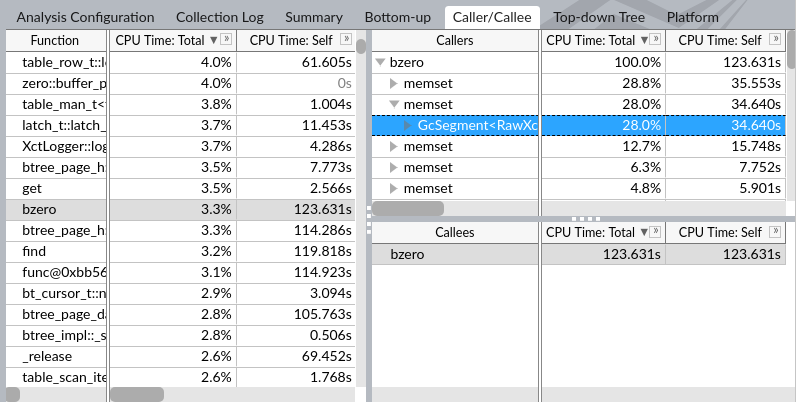
\includegraphics[width = \textwidth]{data/bzero.png}%
        }
        \vspace{.75em}
        \caption[The VTune™ Profiler uncovers unnecessary memory erasure]{The ``Caller/Callee'' tab of an \textit{Intel® VTune™ Profiler} analysis can be used to find code that consumes a significant amount of CPU time.}
        \label{fig:bzero}
    \end{figure}
\end{@empty}

    Finding \emph{small blocks of code} that take up an \emph{unexpectedly large amount of computing time} (or other resources) is probably the most common and basic application of software tracing and profiling.

    The screenshot in figure \ref{fig:bzero} shows part of the ``Caller/Callee'' tab of the \textit{Intel® VTune™ Profiler} analysis of the multithreaded execution of \textit{TPC-C} on \textit{Zero}. The DBS spends \SI{3.3}{\percent} (including benchmark code etc.) of CPU time in \lstinline|bzero|, which \emph{erases memory areas}. Such a call is a good candidate to find unnecessarily used CPU cycles, because such a call is not needed if e.g. the respective memory area is not reused without initialization.

\begin{@empty}
    \begin{code}[h!]
        \begin{lstlisting}[numbers = left, language = C++]
struct GcSegment {
    /* ... */
    void recycle() {
            owner = 0;
            allocated_objects = 0;
            ::memset(objects, 0, sizeof(T) * total_objects);
    }
    /* ... */
}
        \end{lstlisting}
        \caption[Source code with unnecessary memory erasure]{The member function \lstinline|GcSegment::recycle| does unnecessarily erase a memory area.}
        \label{lst:bzero}
    \end{code}
\end{@empty}

    This is the case for the caller \lstinline|GcSegment<RawXct>::recycle| which is responsible for \SI{28}{\percent} of the CPU time spent running \lstinline|bzero|. Listing \ref{lst:bzero} shows the implementation of this member function. As soon as an object of class \lstinline|GcSegment| is no longer needed, it is prepared for later reuse by overwriting all its member variables with zero. \lstinline|bzero| is called by \lstinline|memset| on line 7 because it is called to write zeros into a given memory area. But since it can be guaranteed that no part of the member variable \lstinline|objects| is accessed after reuse before it is reinitialized, this call is unnecessary and a waste of CPU time.

\begin{@empty}
    \pgfplotsset{%
        every axis/.append style = {
            xlabel = {$\text{Transaction throughput }\left[\si{1\per\minute}\right]$},
            xlabel near ticks,
            x label style = {font = \small},
            xticklabel style = {font = \scriptsize},
            xmode = normal,
            xmin = 0,
            scaled x ticks = false,
            xbar = .8pt,
            ymin = -0.75,
            ymax = 1.75,
            bar width = 1.5em,
            ytick style = {draw = none},
            ytick = {0, 1},
            yticklabels = {Optimized, Baseline},
            y tick label style = {align = center,
                                  font = \footnotesize},
            ylabel near ticks,
            y label style = {font = \small},
            xmajorgrids = true,
            width = \textwidth,
            height = .2\textheight
        }
    }

    \begin{figure}[ht!]
        \centering
        \begin{tikzpicture}
            \begin{axis}
                \addplot[draw = Cyan, fill = Cyan!50] coordinates
                {(889279.6, 0) (883277.13, 1)};
            \end{axis}
        \end{tikzpicture}
        \caption[Transaction throughput without unnecessary bzero calls]{Transaction throughput of the \nameref{subsec:random} page replacement algorithm before and after removing unnecessary calls to \lstinline|bzero| (memory erasure) for the \textit{TPC-C} benchmark on 100 warehouses}
        \label{fig:bzerothroughput}
    \end{figure}
\end{@empty}

    Figure \ref{fig:bzero} shows the transaction throughput of \textit{Zero} when running the \textit{TPC-C} Benchmarks before and after removing the mentioned call of \lstinline|bzero|. Both versions use the RANDOM page replacement algorithm and do not use the pointer swizzling technique from subsection \ref{subsec:looking_glass_swizzling}. After saving these $\SI{3.3}{\percent} \cdot \SI{28}{\percent} = \SI{0.924}{\percent}$ of CPU cycles a \SI{\approx 0.67}{\percent} higher transaction throughput can be achieved.

\section{Conclusion} \label{sec:looking_glass_outro}

    While the measurements from ``OLTP through the Looking Glass, and What We Found There'' were driven by the idea of \emph{omitting certain guarantees and features} provided by relational DBMSs, the measurements for section \ref{sec:looking_glass} had the goal of \emph{optimizing certain components} of a DBMS. Using the \emph{tracing} and \emph{profiling} tool \textit{Intel® VTune™ Profiler} it was shown that, depending on the workload, different DBMS components require the largest proportion of CPU cycles. When many small transactions are executed, the transaction manager becomes a bottleneck, but with a balanced workload such as \textit{TPC-C}, key comparisons in the B-tree consume most CPU time.

    These results suggest an optimization of the \emph{transaction manager}. Since most of the CPU time was spent on spinning a spinlock, the complete removal of such a global latch would be an enormous optimization, making this component much more scalable. Optimizations in the \emph{B-tree} are---as demonstrated here again---also always beneficial, especially when executing \textit{TPC-C}. Even though \textit{Zero} uses the well optimized Foster B-tree---many other approaches to optimize B+trees are known. Some of them are described by Goetz Graefe in his book ``Modern B-tree techniques'' \cite{Graefe:2011}.

    When executing \textit{TPC-C}, the \emph{buffer pool} used unexpectedly much CPU time, considering that (almost) all accessed DB pages were in memory during the whole measurement. Therefore, an optimization of the buffer pool like the \emph{pointer swizzling} technique proposed by Graefe et al. in \cite{Graefe:2014} looks promising. However, the performance evaluation of the technique in subsection \ref{subsec:looking_glass_swizzling} showed a decrease in transaction throughput when applied. However, subsection \ref{subsec:looking_glass_bzero} showed that \emph{removing a single line of code} can be enough to improve transaction throughput by \SI{\approx 0.67}{\percent}, which is remarkable given the ease of the change. But as long as the quality of the implementation of a DBMS is not extremely poor, not much unnecessary code should be found that requires a considerable amount of CPU cycles, so such success should not be easily repeatable.
